\documentclass[11pt,a4paper]{article}
% Build: python scripts/make_dl_report_tables.py && cd docs/dl_report && tectonic dl_report.tex   (or: make dl-report)
% Every number below is a macro or table generated from results/ by scripts/make_dl_report_tables.py.

\usepackage[T1]{fontenc}
\usepackage{lmodern}
\usepackage[a4paper,margin=2.4cm]{geometry}
\usepackage{microtype}
\usepackage{amsmath,amssymb,bm}
\usepackage{graphicx}
\usepackage{booktabs,tabularx,array,multirow}
\usepackage{caption,subcaption}
\usepackage{enumitem}
\usepackage{xcolor}
\usepackage{colortbl}
\usepackage{float}
\usepackage[section]{placeins}
\usepackage{fancyhdr}
\usepackage{tikz}
\usetikzlibrary{positioning,arrows.meta,fit,backgrounds,calc}
\usepackage[numbers,sort&compress]{natbib}
\usepackage[colorlinks=true,linkcolor=blue!50!black,citecolor=blue!50!black,urlcolor=blue!50!black,
  pdftitle={Traffic Flow Prediction with Graph Neural Networks: DL project report},
  pdfauthor={Team T036: Harsh Raj, Manas Saxena, Adil Mirza, Augustya Purohit, Sumit Yadav},
  pdfsubject={Graph attention, diffusion convolution and a hybrid tree corrector on METR-LA},
  pdfkeywords={traffic forecasting, graph neural networks, GATv2, DCRNN, METR-LA}]{hyperref}

\graphicspath{{../figures/}}
\newcommand{\PersistMAEFifteen}{3.49}
\newcommand{\PersistRMSEFifteen}{6.39}
\newcommand{\PersistMAPEFifteen}{8.6}
\newcommand{\PersistMAEThirty}{4.20}
\newcommand{\PersistRMSEThirty}{8.01}
\newcommand{\PersistMAPEThirty}{10.8}
\newcommand{\PersistMAESixty}{5.37}
\newcommand{\PersistRMSESixty}{10.29}
\newcommand{\PersistMAPESixty}{14.5}
\newcommand{\PersistPeakSixty}{8.32}
\newcommand{\PersistOffpeakSixty}{4.62}
\newcommand{\XgbMAEFifteen}{3.02}
\newcommand{\XgbRMSEFifteen}{5.47}
\newcommand{\XgbMAPEFifteen}{8.2}
\newcommand{\XgbMAEThirty}{3.51}
\newcommand{\XgbRMSEThirty}{6.41}
\newcommand{\XgbMAPEThirty}{10.1}
\newcommand{\XgbMAESixty}{4.01}
\newcommand{\XgbRMSESixty}{7.28}
\newcommand{\XgbMAPESixty}{12.0}
\newcommand{\XgbPeakSixty}{6.22}
\newcommand{\XgbOffpeakSixty}{3.31}
\newcommand{\XgbNbMAEFifteen}{2.91}
\newcommand{\XgbNbRMSEFifteen}{5.17}
\newcommand{\XgbNbMAPEFifteen}{7.7}
\newcommand{\XgbNbMAEThirty}{3.42}
\newcommand{\XgbNbRMSEThirty}{6.17}
\newcommand{\XgbNbMAPEThirty}{9.6}
\newcommand{\XgbNbMAESixty}{3.95}
\newcommand{\XgbNbRMSESixty}{7.14}
\newcommand{\XgbNbMAPESixty}{11.7}
\newcommand{\XgbNbPeakSixty}{6.07}
\newcommand{\XgbNbOffpeakSixty}{3.29}
\newcommand{\LstmMAEFifteen}{2.97}
\newcommand{\LstmRMSEFifteen}{5.84}
\newcommand{\LstmMAPEFifteen}{8.0}
\newcommand{\LstmMAEThirty}{3.55}
\newcommand{\LstmRMSEThirty}{7.20}
\newcommand{\LstmMAPEThirty}{10.3}
\newcommand{\LstmMAESixty}{4.35}
\newcommand{\LstmRMSESixty}{8.84}
\newcommand{\LstmMAPESixty}{13.5}
\newcommand{\LstmPeakSixty}{6.96}
\newcommand{\LstmOffpeakSixty}{3.66}
\newcommand{\StgatMAEFifteen}{2.84}
\newcommand{\StgatRMSEFifteen}{5.43}
\newcommand{\StgatMAPEFifteen}{7.5}
\newcommand{\StgatMAEThirty}{3.32}
\newcommand{\StgatRMSEThirty}{6.61}
\newcommand{\StgatMAPEThirty}{9.4}
\newcommand{\StgatMAESixty}{3.95}
\newcommand{\StgatRMSESixty}{7.96}
\newcommand{\StgatMAPESixty}{11.9}
\newcommand{\StgatPeakSixty}{6.07}
\newcommand{\StgatOffpeakSixty}{3.36}
\newcommand{\DcrnnMAEFifteen}{2.64}
\newcommand{\DcrnnRMSEFifteen}{5.17}
\newcommand{\DcrnnMAPEFifteen}{6.8}
\newcommand{\DcrnnMAEThirty}{3.05}
\newcommand{\DcrnnRMSEThirty}{6.34}
\newcommand{\DcrnnMAPEThirty}{8.4}
\newcommand{\DcrnnMAESixty}{3.57}
\newcommand{\DcrnnRMSESixty}{7.67}
\newcommand{\DcrnnMAPESixty}{10.4}
\newcommand{\DcrnnPeakSixty}{5.40}
\newcommand{\DcrnnOffpeakSixty}{3.00}
\newcommand{\HybridMAEFifteen}{2.62}
\newcommand{\HybridRMSEFifteen}{5.11}
\newcommand{\HybridMAPEFifteen}{6.8}
\newcommand{\HybridMAEThirty}{3.01}
\newcommand{\HybridRMSEThirty}{6.20}
\newcommand{\HybridMAPEThirty}{8.4}
\newcommand{\HybridMAESixty}{3.47}
\newcommand{\HybridRMSESixty}{7.30}
\newcommand{\HybridMAPESixty}{10.3}
\newcommand{\HybridPeakSixty}{5.20}
\newcommand{\HybridOffpeakSixty}{2.95}
\newcommand{\RfMAEFifteen}{3.08}
\newcommand{\RfRMSEFifteen}{5.62}
\newcommand{\RfMAPEFifteen}{8.3}
\newcommand{\RfMAEThirty}{3.68}
\newcommand{\RfRMSEThirty}{6.71}
\newcommand{\RfMAPEThirty}{10.6}
\newcommand{\RfMAESixty}{4.45}
\newcommand{\RfRMSESixty}{7.85}
\newcommand{\RfMAPESixty}{13.5}
\newcommand{\RfPeakSixty}{7.08}
\newcommand{\RfOffpeakSixty}{3.62}
\newcommand{\DcrnnGainFifteen}{12.3}
\newcommand{\DcrnnGainThirty}{13.1}
\newcommand{\DcrnnGainSixty}{11.0}
\newcommand{\StgatGainFifteen}{5.8}
\newcommand{\StgatGainThirty}{5.4}
\newcommand{\StgatGainSixty}{1.3}
\newcommand{\HybridGainFifteen}{13.0}
\newcommand{\HybridGainThirty}{14.2}
\newcommand{\HybridGainSixty}{13.3}
\newcommand{\XgbNbGainFifteen}{3.5}
\newcommand{\XgbNbGainThirty}{2.6}
\newcommand{\XgbNbGainSixty}{1.4}
\newcommand{\HybridOverDcrnnFifteen}{0.8}
\newcommand{\HybridOverDcrnnThirty}{1.2}
\newcommand{\HybridOverDcrnnSixty}{2.6}
\newcommand{\PeakGainDcrnn}{13.3}
\newcommand{\PeakGainHybrid}{16.5}
\newcommand{\TestDays}{24}
\newcommand{\StgatSixtyPBoot}{0.021}
\newcommand{\StgatSixtyPDm}{0.061}
\newcommand{\StgatSixtyDays}{16}
\newcommand{\HybridMinDays}{23}
\newcommand{\RefFifteen}{2.63}
\newcommand{\PubFifteen}{2.67}
\newcommand{\RefThirty}{3.03}
\newcommand{\PubThirty}{3.08}
\newcommand{\RefSixty}{3.54}
\newcommand{\PubSixty}{3.56}
\newcommand{\RefWorstPct}{1.5}
\newcommand{\AttSelfNormal}{16.5}
\newcommand{\AttUpNormal}{31.5}
\newcommand{\AttDownNormal}{52.0}
\newcommand{\AttSelfAhead}{11.8}
\newcommand{\AttUpAhead}{25.7}
\newcommand{\AttDownAhead}{62.5}
\newcommand{\AttSensors}{163}
\newcommand{\AttShifted}{149}
\newcommand{\AttWindows}{18\,955}
\newcommand{\DegGainLow}{4.3}
\newcommand{\DegGainHigh}{12.8}
\newcommand{\OnsetXgbFifteen}{16.2}
\newcommand{\OnsetXgbThirty}{20.1}
\newcommand{\OnsetXgbSixty}{19.1}
\newcommand{\OnsetDcrnnFifteen}{13.3}
\newcommand{\OnsetDcrnnThirty}{18.2}
\newcommand{\OnsetDcrnnSixty}{20.7}
\newcommand{\OnsetHybridFifteen}{13.3}
\newcommand{\OnsetHybridThirty}{18.2}
\newcommand{\OnsetHybridSixty}{20.2}
\newcommand{\OnsetStgatFifteen}{15.5}
\newcommand{\OnsetStgatThirty}{21.1}
\newcommand{\OnsetStgatSixty}{23.6}
\newcommand{\OnsetTargets}{27\,023}
\newcommand{\TestOnsets}{3\,911}
\newcommand{\MapTime}{2012-06-08 16:30}
\newcommand{\MapCongested}{103}
\newcommand{\MapXgbCaught}{75}
\newcommand{\MapGraphCaught}{88}
\newcommand{\MapXgbLevel}{81.2}
\newcommand{\MapGraphLevel}{86.1}
\newcommand{\MapSensorsBetter}{198}
\newcommand{\MapMedianGain}{0.32}
\newcommand{\TsDay}{2012-06-13}
\newcommand{\TsSensors}{15}
\newcommand{\TsKm}{15.6}
\newcommand{\AblNoGraphSixty}{4.35}
\newcommand{\AblNoGraphDelta}{0.40}
\newcommand{\AblFwdSixty}{4.05}
\newcommand{\AblFwdDelta}{0.10}
\newcommand{\AblBwdSixty}{4.02}
\newcommand{\AblBwdDelta}{0.07}
\newcommand{\AblUndirSixty}{4.04}
\newcommand{\AblUndirDelta}{0.09}
\newcommand{\AblRandomSixty}{4.18}
\newcommand{\AblRandomDelta}{0.22}
\newcommand{\AblOneLayerSixty}{4.11}
\newcommand{\AblOneLayerDelta}{0.15}
\newcommand{\AblNoDropSixty}{3.92}
\newcommand{\AblNoDropDelta}{-0.03}
\newcommand{\AblDcrnnFwdSixty}{3.72}
\newcommand{\AblDcrnnFwdDelta}{0.15}
\newcommand{\AblDcrnnKoneSixty}{3.57}
\newcommand{\AblDcrnnKoneDelta}{0.00}
\newcommand{\StgatParams}{65\,420}
\newcommand{\DcrnnParams}{377\,153}
\newcommand{\HybFitWindows}{2\,562}
\newcommand{\HybStopWindows}{855}
\newcommand{\PropDownFirst}{156}
\newcommand{\PropUpFirst}{41}
\newcommand{\PropLag}{10}
\newcommand{\PropKmh}{16}
\newcommand{\GraphEdges}{1\,515}
\newcommand{\GraphDegree}{7.32}
\newcommand{\ZeroPct}{8.1}
\newcommand{\NTests}{53}
\newcommand{\BlendWFifteen}{0.89}
\newcommand{\BlendWSixty}{0.84}
\newcommand{\CorrTopShare}{29}

\makeatletter\newcommand{\tabinput}[1]{\@@input #1 }\makeatother

\definecolor{navy}{HTML}{1F3A5F}
\definecolor{accent}{HTML}{2A78D6}
\definecolor{soft}{HTML}{EEF3F9}
\definecolor{good}{HTML}{2E7D32}
\definecolor{warn}{HTML}{B26A00}

\captionsetup{font=small,labelfont={bf,color=navy},skip=6pt}
\setlist{itemsep=2pt,topsep=4pt}
\setlength{\parindent}{0pt}
\setlength{\parskip}{6pt}
\setlength{\emergencystretch}{2em}
\renewcommand{\arraystretch}{1.18}
\pagestyle{fancy}
\fancyhf{}
\fancyhead[L]{\small\color{navy} Traffic flow forecasting on METR-LA}
\fancyhead[R]{\small\color{navy} Deep-learning phase report}
\fancyfoot[C]{\small\thepage}
\renewcommand{\headrulewidth}{0.4pt}

\newcommand{\repository}{\url{https://github.com/ManasSaxena14/TrafficFlowControl_AIML-DL_T036}}
\newcommand{\dashboard}{\url{https://trafficflowamldl.streamlit.app}}
\newcommand{\mph}{~mph}

% a shaded key-result box
\newenvironment{keybox}[1]{\par\smallskip\noindent\begin{tikzpicture}\node[fill=soft,draw=accent,line width=0.6pt,rounded corners=3pt,
  inner sep=8pt,text width=\dimexpr\linewidth-17.2pt\relax]\bgroup{\color{navy}\textbf{#1}}\par\smallskip}{\egroup;\end{tikzpicture}\par\smallskip}

\tikzset{
  blk/.style={draw=navy,fill=soft,rounded corners=2pt,align=center,font=\small,minimum height=9mm,inner sep=4pt},
  dark/.style={draw=navy,fill=navy,text=white,rounded corners=2pt,align=center,font=\small\bfseries,minimum height=9mm,inner sep=4pt},
  arr/.style={-{Stealth[length=2.2mm]},thick,draw=navy},
}

\begin{document}

%=====================================================================  title page
\begin{titlepage}
\centering
\vspace*{1.2cm}
{\large\color{accent}\textsc{Project 4: Traffic Flow Control}\par}
\vspace{0.6cm}
{\LARGE\bfseries\color{navy} Traffic Flow Prediction and Signal Control\\[4pt] via Graph Attention Networks and Flow Models\par}
\vspace{0.5cm}
{\Large Deep-Learning Phase Report\par}
\vspace{0.3cm}
{\large Graph neural networks over the road graph, a hybrid tree corrector,\\ and a leak-free, significance-tested comparison on METR-LA\par}
\vspace{1.4cm}

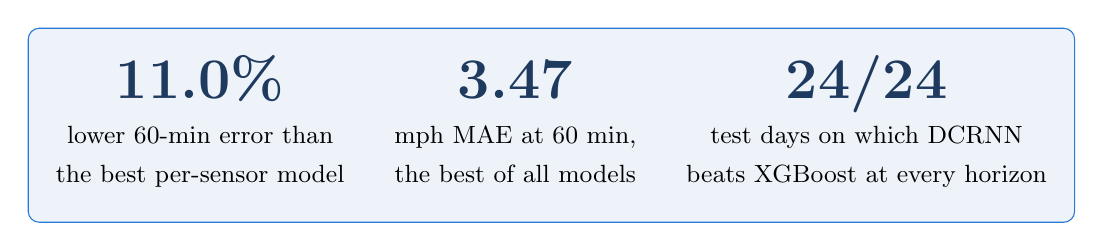
\begin{tikzpicture}
\node[fill=soft,draw=accent,rounded corners=4pt,inner sep=10pt,align=center]{
  \setlength{\tabcolsep}{9pt}\begin{tabular}{@{}ccc@{}}
  {\huge\bfseries\color{navy}\DcrnnGainSixty\%} & {\huge\bfseries\color{navy}\HybridMAESixty} & {\huge\bfseries\color{navy}\TestDays/\TestDays}\\[2pt]
  \small lower 60-min error than & \small mph MAE at 60 min, & \small test days on which DCRNN\\
  \small the best per-sensor model & \small the best of all models & \small beats XGBoost at every horizon
  \end{tabular}};
\end{tikzpicture}

\vspace{1.6cm}
{\large\bfseries Team T036\par}
\vspace{0.2cm}
\begin{tabular}{ll}
Harsh Raj & 2401010180\\
Manas Saxena & 2401010260\\
Adil Mirza & 2401020005\\
Augustya Purohit & 2401010114\\
Sumit Yadav & 2401010464
\end{tabular}

\vspace{0.6cm}
Newton School of Technology, Rishihood University\par
\vfill
{\small Source code, results and data pipeline: \repository\\
Interactive results dashboard: \dashboard\par}
\end{titlepage}

%=====================================================================  abstract
\begin{abstract}
\noindent
Traffic congestion is a network phenomenon: a jam forms at a bottleneck and travels backwards along the freeway, so the
most useful signal for one road sensor often sits at its neighbours. The applied-machine-learning (AML) phase of this
project built leak-free per-sensor baselines on METR-LA (207 Los Angeles freeway sensors, 5-minute speeds) and measured
what they miss. This report covers the deep-learning (DL) phase, which asks whether models that read the road graph
close that gap, by how much, and why.
We train two graph neural networks on exactly the same windows, mask and metric code as the baselines: STGAT, a
spatio-temporal graph attention network whose GATv2 attention runs over both directions of every road link, and a
PyTorch port of the diffusion convolutional recurrent network (DCRNN). We then propose a hybrid that keeps DCRNN as the
backbone and lets a small, regularised XGBoost model learn its systematic error on held-out data.
Under a strict chronological protocol, DCRNN lowers the test mean absolute error of the best per-sensor model (XGBoost)
by \DcrnnGainFifteen\%, \DcrnnGainThirty\% and \DcrnnGainSixty\% at 15, 30 and 60 minutes, on every one of the
\TestDays{} test days (paired day-level bootstrap and Diebold--Mariano tests, $p<0.0001$). The hybrid is the best model
overall, at \HybridMAEFifteen, \HybridMAEThirty{} and \HybridMAESixty\mph, a further \HybridOverDcrnnSixty\% below DCRNN at
60 minutes, and the best model at weekday peak hours. Nine ablations show that the gain comes from the real road graph
(a random graph of the same size is clearly worse) and from listening to downstream neighbours, and the trained
attention shifts downstream when a slowdown is approaching. Our DCRNN port reproduces the published METR-LA numbers to
within \RefWorstPct\%. We close with congestion maps, an error map, a time--space diagram and an honest account of what
was not done: signal control was not simulated, and nothing in this project controls real traffic.
\end{abstract}

\vspace{0.4cm}
\begin{keybox}{Outcomes at a glance}
\begin{itemize}[leftmargin=1.2em]
\item \textbf{The graph helps, significantly.} DCRNN beats the tuned XGBoost by 11--13\% at every horizon, on all \TestDays{} test days.
\item \textbf{The hybrid is best.} DCRNN + XGBoost residual corrector: \HybridMAEFifteen{} / \HybridMAEThirty{} / \HybridMAESixty\mph{} MAE at 15 / 30 / 60 min; \PeakGainHybrid\% lower peak-hour error than XGBoost.
\item \textbf{The road matters.} No graph or a random graph removes most of the gain; downstream messages matter more than upstream ones.
\item \textbf{The attention is interpretable.} STGAT moves its attention downstream (\AttDownNormal\% $\rightarrow$ \AttDownAhead\%) when a slowdown is 30 minutes away, for \AttShifted{} of \AttSensors{} sensors.
\item \textbf{The implementation is faithful.} Our DCRNN reaches \RefFifteen{} / \RefThirty{} / \RefSixty\mph{} under the reference protocol against the published \PubFifteen{} / \PubThirty{} / \PubSixty.
\end{itemize}
\end{keybox}

\clearpage
\setcounter{tocdepth}{2}
\tableofcontents
\clearpage

%=====================================================================
\section{Introduction}\label{sec:intro}

\subsection{Motivation}
Short-term forecasts of traffic speed, from five minutes to an hour ahead, feed route guidance, incident response and
signal timing. The simplest way to forecast a road network is one segment at a time: each sensor is predicted from its
own recent history, the time of day and a few static descriptors. Such models can be very strong; in the AML phase a
tuned XGBoost model per horizon was the best of six baselines. But a per-sensor model cannot see a jam that is forming one
link away. On METR-LA congestion travels \emph{backwards}: on strongly coupled links the downstream sensor slows first
\PropDownFirst{} times against \PropUpFirst{} for the upstream one, with a median lag of \PropLag{} minutes and an
implied shock-wave speed of about \PropKmh{}~km/h (Figure~\ref{fig:prop}).

Graph neural networks (GNNs) read the road network directly and are the standard approach on benchmarks such as
METR-LA~\citep{li2018dcrnn,yu2018stgcn,wu2019graphwavenet}. Reported gains, however, are usually measured against weak
baselines, under window-level splits in which training and validation targets overlap, and as a single average. This
report measures the gain against strong baselines under a strict protocol, tests it for significance, and asks where it
comes from.

\begin{figure}[htbp]
\centering
\includegraphics[width=0.86\linewidth]{fig05d_propagation_example.png}
\caption{A jam reaches the downstream sensor first and the upstream sensor, 1.5~km back, about 10 minutes later. A
per-sensor model at the upstream sensor cannot see it coming; a graph model can. (Training period; from the AML phase.)}
\label{fig:prop}
\end{figure}

\subsection{Project brief and scope of this report}
The brief (Project 4, \emph{Traffic Flow Control}) asks for a hybrid logic: segment-level machine-learning baselines
first, a measured gap second, and network-aware graph learning third, compared fairly with chronological splits, MAE,
RMSE and MAPE by horizon, equal history windows and peak versus off-peak periods, with congestion maps as the expected
deliverable and signal control as an optional, simulated-only experiment. The AML phase delivered the first two steps
and is documented in its own report (\texttt{docs/report/report.pdf}); it is summarised in Section~\ref{sec:aml} only as
far as the DL phase builds on it. This report covers the third step and the final comparison.

\subsection{Research questions}
\begin{enumerate}[label=\textbf{RQ\arabic*.},leftmargin=3em]
\item Does a graph neural network over the fixed road graph forecast speed more accurately than the best per-sensor model, at every horizon, and is the difference statistically reliable?
\item Where does the gain come from: the road graph itself, the direction of information flow, the number of hops, or just a larger model?
\item Where in the network and when in the day does the graph help most?
\item Are graph models and tree models complementary, and can a hybrid exploit it without leaking test information?
\item What does the attention of a graph attention network learn about the road?
\end{enumerate}

\subsection{Contributions}
\begin{itemize}
\item \textbf{STGAT}, a compact spatio-temporal graph attention network (\StgatParams{} parameters) with bidirectional,
direction-aware edges motivated by the measured upstream propagation of congestion; its GATv2 layer is written in plain
PyTorch and tested to be numerically identical to PyTorch Geometric's \texttt{GATv2Conv}.
\item \textbf{A faithful PyTorch DCRNN} (\DcrnnParams{} parameters) that reproduces the published METR-LA results.
\item \textbf{A justified ML+DL hybrid}: DCRNN plus a per-horizon, heavily regularised XGBoost residual corrector fitted
only on the validation block, the best model of the project.
\item \textbf{A fair comparison} of ten models on one test block with day-level paired bootstrap and Diebold--Mariano
tests, nine ablations, a breakdown by connectivity and around congestion onsets, and an inspection of the attention.
\item \textbf{Congestion maps}, an error map, a time--space diagram and an animated map, every number in this report
generated from the result files in the repository.
\end{itemize}

%=====================================================================
\section{Background and related work}\label{sec:related}

\subsection{Per-sensor forecasting}
Classical approaches forecast each location independently: historical averages by time of day, linear models such as
ridge regression~\citep{hoerl1970ridge}, and tree ensembles such as Random Forest~\citep{breiman2001rf} and gradient
boosting with XGBoost~\citep{chen2016xgboost} on engineered lags and calendar features. Recurrent networks, the
LSTM~\citep{hochreiter1997lstm} and GRU~\citep{cho2014gru}, learn temporal patterns from raw sequences but, when shared
across sensors, still treat each sensor in isolation.

\subsection{Graph neural networks for traffic}
A road network is naturally a graph whose nodes are sensors and whose edges are road links. Spectral and spatial graph
convolutions~\citep{kipf2017gcn} aggregate each node's neighbours with fixed normalised weights.
\textbf{DCRNN}~\citep{li2018dcrnn} models traffic as a diffusion process on a \emph{directed} graph, using forward and
backward random walks as graph convolutions inside a GRU encoder--decoder trained with scheduled
sampling~\citep{bengio2015scheduled}; it introduced the METR-LA benchmark and its protocol.
STGCN~\citep{yu2018stgcn} replaces recurrence with temporal convolutions, Graph WaveNet~\citep{wu2019graphwavenet} adds
dilated convolutions and a learned adaptive adjacency, and attention-based models such as
ASTGCN~\citep{guo2019astgcn} and GMAN~\citep{zheng2020gman} learn spatial and temporal attention.

\subsection{Graph attention}
Graph attention networks (GAT)~\citep{velickovic2018gat} replace fixed neighbour weights with learned,
feature-dependent attention coefficients, so a node can weigh the neighbours that matter now. Brody et
al.~\citep{brody2022gatv2} showed that the original GAT computes only a \emph{static} ranking of neighbours (the same
for every query node) and proposed GATv2, which applies the nonlinearity before the attention vector and is strictly
more expressive. STGAT uses GATv2 with edge features.

\subsection{Hybrids, leakage and evaluation}
Stacked generalisation~\citep{wolpert1992stacking} trains a second-level model on \emph{held-out} predictions of
first-level models; our hybrid applies this idea to let trees correct a GNN. Leakage through overlapping windows or
preprocessing statistics computed on the full series is a known source of optimistic results~\citep{kaufman2012leakage}.
MAE, RMSE and MAPE answer different questions~\citep{hyndman2006measures}. Forecasts are compared with the
Diebold--Mariano test~\citep{diebold1995dm} with the small-sample correction of Harvey et al.~\citep{harvey1997hln}, and
with a paired bootstrap~\citep{efron1993bootstrap}.

\subsection{Signal control}
Signal-control studies use microscopic simulators such as SUMO or CityFlow~\citep{zhang2019cityflow}. METR-LA covers
freeways, which have no signals, so any control study on it would be a simulation of a synthetic network.

\begin{table}[htbp]
\centering
\caption{Literature map: the role of each reference in the DL phase.}
\label{tab:litmap}
\small
\begin{tabularx}{\linewidth}{@{}p{4.3cm}X@{}}
\toprule
Reference & Used in this phase for \\
\midrule
Li et al.~\citep{li2018dcrnn} & DCRNN model, data and graph, reference protocol to reproduce; motivates the direction ablations \\
Veli\v{c}kovi\'c et al.~\citep{velickovic2018gat}; Brody et al.~\citep{brody2022gatv2} & graph attention in STGAT (GATv2 layer) \\
Kipf and Welling~\citep{kipf2017gcn}; Yu et al.~\citep{yu2018stgcn}; Wu et al.~\citep{wu2019graphwavenet} & related graph models; learned adjacency as an extension \\
Guo et al.~\citep{guo2019astgcn}; Zheng et al.~\citep{zheng2020gman} & attention-based traffic models, context for STGAT \\
Cho et al.~\citep{cho2014gru}; Hochreiter and Schmidhuber~\citep{hochreiter1997lstm} & GRU temporal encoder; no-graph LSTM control \\
Bengio et al.~\citep{bengio2015scheduled} & scheduled sampling in the DCRNN decoder \\
Srivastava et al.~\citep{srivastava2014dropout}; Ba et al.~\citep{ba2016layernorm}; Kingma and Ba~\citep{kingma2015adam} & regularisation and optimisation \\
Wolpert~\citep{wolpert1992stacking}; Chen and Guestrin~\citep{chen2016xgboost} & design of the hybrid residual corrector \\
Diebold and Mariano~\citep{diebold1995dm}; Harvey et al.~\citep{harvey1997hln}; Efron and Tibshirani~\citep{efron1993bootstrap} & day-level significance tests \\
Kaufman et al.~\citep{kaufman2012leakage}; Hyndman and Koehler~\citep{hyndman2006measures} & leak-free protocol; reading of MAE, RMSE and MAPE \\
Paszke et al.~\citep{paszke2019pytorch}; Fey and Lenssen~\citep{fey2019pyg} & implementation; reference for the attention-layer equivalence test \\
Zhang et al.~\citep{zhang2019cityflow} & scope of the optional, simulation-only signal control \\
\bottomrule
\end{tabularx}
\end{table}

%=====================================================================
\section{Starting point: the AML phase and the measured gap}\label{sec:aml}
The DL phase starts from the AML phase's pipeline, baselines and findings, which are unchanged here.

\textbf{Baselines.} Six models share one 46-column feature table per sensor and time (12 speed lags, rolling statistics,
recent change, missing-value flags, cyclic time, segment statistics): persistence, historical average, ridge per sensor,
a multi-output Random Forest, XGBoost per horizon and an LSTM with weights shared across sensors and no graph. XGBoost is
the strongest, at \XgbMAEFifteen{} / \XgbMAEThirty{} / \XgbMAESixty\mph{} test MAE at 15 / 30 / 60 minutes.

\textbf{The gap.} Four experiments showed that (H1) error grows with the horizon; (H2) in the 30 minutes after a
congestion onset XGBoost's error is several times larger (\TestOnsets{} onsets in the test block); (H3) the residuals of
road-linked sensors are correlated while those of unconnected sensors are not; and (H4) adding hand-made one-hop
neighbour speeds lowers error at every horizon (to \XgbNbMAEFifteen{} / \XgbNbMAEThirty{} / \XgbNbMAESixty\mph), more
from downstream than from upstream neighbours, but only partly. The missing information is spatial, and one-hop features
capture only part of it: the case for a graph model.

\textbf{Hypotheses for the DL phase.} Building on H1--H4 and the literature, we test:
\begin{enumerate}[label=\textbf{H\arabic*},start=5,leftmargin=2.6em]
\item A graph model beats the best per-sensor model at every horizon, reliably across test days.
\item The gain comes from the real road graph, not from extra capacity: without a graph or with a random graph it disappears.
\item Information from downstream neighbours is worth more than from upstream ones.
\item The gain is larger for well-connected sensors and right after congestion starts.
\item Graph and tree models are complementary: a leak-free hybrid improves on the best graph model.
\end{enumerate}

%=====================================================================
\section{Data and leak-free protocol}\label{sec:data}

\subsection{METR-LA and the road graph}
METR-LA~\citep{jagadish2014bigdata,li2018dcrnn} holds 34\,272 five-minute speed readings for 207 loop detectors on Los
Angeles freeways, from 1 March to 27 June 2012. The road graph is a directed, weighted adjacency built from driving
distances,
\begin{equation}
W_{ij} = \begin{cases}\exp\!\left(-d_{ij}^2/\sigma^2\right) & \text{if } \exp\!\left(-d_{ij}^2/\sigma^2\right)\ge 0.1,\\ 0 & \text{otherwise,}\end{cases}
\end{equation}
where $d_{ij}$ is the road distance from sensor $i$ to sensor $j$ and $\sigma$ the standard deviation of all distances.
$W_{ij}>0$ means traffic drives from $i$ to $j$, so $i$ is \emph{upstream} of $j$. The graph has \GraphEdges{} directed
links and a mean degree of \GraphDegree. We rebuild $W$ from the raw distances and a test checks that it equals the
supplied matrix. \ZeroPct\% of all readings are 0\mph, which marks a sensor outage, not stopped traffic.

\subsection{Protocol shared by every model}
\begin{itemize}
\item \textbf{Chronological, purged split.} Timestamps are split 70 / 10 / 20\% into train, validation and test blocks;
windows are cut inside each block, so no target timestamp appears in two splits (Table~\ref{tab:splits}).
\item \textbf{Equal history.} Every model sees the last 12 steps (60 minutes) and forecasts the next 12 (5 to 60 minutes).
\item \textbf{Train-only statistics.} The scaler and the imputation table are fitted on training timestamps only.
\item \textbf{Masked outages.} Outages are NaN, never 0\mph. Inputs are forward-filled inside the window (otherwise the
training mean of that sensor and time slot) and carry a mask channel; targets are never imputed and masked targets
contribute nothing to any loss or metric.
\item \textbf{Cyclic time.} Time of day and day of week enter as sine/cosine pairs, plus a weekend flag.
\item \textbf{One evaluation path.} All models are scored by the same masked MAE, RMSE and MAPE functions, in mph, on the
same test windows. Peak hours are weekdays 07:00--09:59 and 16:00--19:59, judged on the timestamp being predicted.
\end{itemize}
Each graph model receives the tensor $\bm X\in\mathbb R^{B\times 12\times 207\times 7}$ (scaled speed, mask, four cyclic
time features, weekend flag) and outputs $\hat{\bm Y}\in\mathbb R^{B\times 12\times 207}$.

\begin{table}[htbp]
\centering
\caption{Chronological splits used by every model (strict protocol).}
\label{tab:splits}
\small
\input{../report/generated/tab_splits.tex}
\end{table}

\begin{figure}[htbp]
\centering
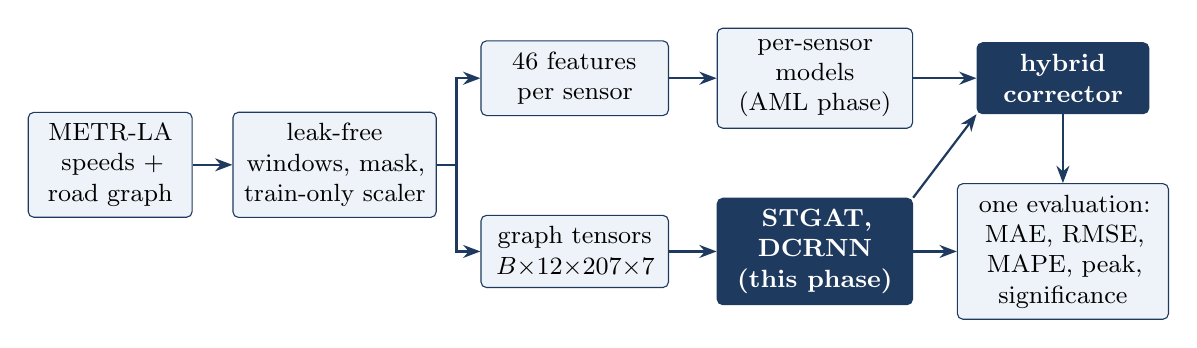
\begin{tikzpicture}[x=1cm,y=1cm]
\node[blk,text width=1.8cm] (raw) at (1.0,0) {METR-LA speeds + road graph};
\node[blk,text width=2.3cm] (pre) at (3.85,0) {leak-free windows, mask, train-only scaler};
\node[blk,text width=2.1cm] (feat) at (6.9,1.1) {46 features per sensor};
\node[blk,text width=2.1cm] (tens) at (6.9,-1.1) {graph tensors $B{\times}12{\times}207{\times}7$};
\node[blk,text width=2.2cm] (ml) at (9.95,1.1) {per-sensor models (AML phase)};
\node[dark,text width=2.2cm] (dl) at (9.95,-1.1) {STGAT, DCRNN (this phase)};
\node[dark,text width=1.9cm] (hy) at (13.1,1.1) {hybrid corrector};
\node[blk,text width=2.4cm] (ev) at (13.1,-1.1) {one evaluation: MAE, RMSE, MAPE, peak, significance};
\draw[arr] (raw) -- (pre);
\draw[arr] (pre.east) -- ++(0.25,0) |- (feat.west);
\draw[arr] (pre.east) -- ++(0.25,0) |- (tens.west);
\draw[arr] (feat) -- (ml); \draw[arr] (tens) -- (dl);
\draw[arr] (ml) -- (hy); \draw[arr] (dl.north east) -- (hy.south west);
\draw[arr] (dl) -- (ev); \draw[arr] (hy) -- (ev);
\end{tikzpicture}
\caption{Pipeline. Both phases share one preprocessing step and one evaluation path; the hybrid combines a graph model
with the per-sensor XGBoost forecasts.}
\label{fig:pipeline}
\end{figure}

%=====================================================================
\section{Models}\label{sec:models}

\subsection{Problem formulation}
Let $x_t\in\mathbb R^{N}$ be the speeds of the $N=207$ sensors at time $t$ and $G=(V,E,W)$ the road graph. A forecaster
learns
\begin{equation}
f:\ \left(x_{t-11},\dots,x_t;\,G\right)\ \mapsto\ \left(\hat x_{t+1},\dots,\hat x_{t+12}\right),
\end{equation}
minimising the masked mean absolute error in mph,
\begin{equation}
\mathcal L = \frac{1}{\sum m}\sum_{s,h,i} m_{s,h,i}\,\bigl|\hat y_{s,h,i}-y_{s,h,i}\bigr|,
\end{equation}
where $m_{s,h,i}=0$ marks an outage. A per-sensor model is the special case in which sensor $i$'s forecast depends only on
sensor $i$'s inputs; a graph model may use any sensor's inputs, through $G$.

\subsection{STGAT: spatio-temporal graph attention network}\label{sec:stgat}
STGAT separates time and space (Figure~\ref{fig:stgat}).
\begin{enumerate}
\item \textbf{Temporal encoder.} A two-layer GRU~\citep{cho2014gru} with 64 hidden units, shared by all sensors, reads
each sensor's 12 input steps and returns a summary $h_i\in\mathbb R^{64}$ of its recent trajectory.
\item \textbf{Spatial attention.} Two GATv2 layers~\citep{brody2022gatv2} with 4 heads let each sensor attend to its road
neighbours' summaries:
\begin{align}
e_{ij} &= \bm a^{\top}\,\mathrm{LeakyReLU}\!\left(W_r h_i + W_l h_j + W_e\,\epsilon_{ji}\right),\\
\alpha_{ij} &= \frac{\exp(e_{ij})}{\sum_{k\in\mathcal N(i)}\exp(e_{ik})},\qquad
h_i' = \mathrm{LayerNorm}\Bigl(h_i + \mathrm{Dropout}\bigl(\mathrm{ELU}\bigl(\textstyle\sum_{j\in\mathcal N(i)}\alpha_{ij}W_l h_j\bigr)\bigr)\Bigr),
\end{align}
with residual connections and layer normalisation~\citep{ba2016layernorm}.
\item \textbf{Head.} An MLP maps $[h_i,\,h_i']$ to the 12 horizons as a \emph{change} from the last observed speed.
\end{enumerate}

\textbf{Bidirectional, direction-aware edges.} Message passing on the raw matrix sends messages only from upstream to
downstream, so a sensor would hear only its upstream neighbours. Because jams arrive from downstream
(Figure~\ref{fig:prop}), every link is added in both directions with edge features $\epsilon=[W_{ij},\ \text{is\_reverse}]$,
plus a self-loop, and the attention learns how much each direction is worth.

\textbf{Design choice: attend once, after the encoder.} Attending at every input step costs 12 graph passes per window;
attending once on the GRU summaries, which already hold each neighbour's recent trajectory, is about 8$\times$ cheaper
per training batch and made three seeds and seven STGAT ablations affordable.

\textbf{Implementation.} The GATv2 layer is written in plain PyTorch~\citep{paszke2019pytorch} over an edge list shared by
all graphs in a batch, so it runs on CPU, CUDA and Apple-silicon GPUs; a unit test checks that it matches PyTorch
Geometric's \texttt{GATv2Conv}~\citep{fey2019pyg} to numerical precision.

\begin{figure}[htbp]
\centering
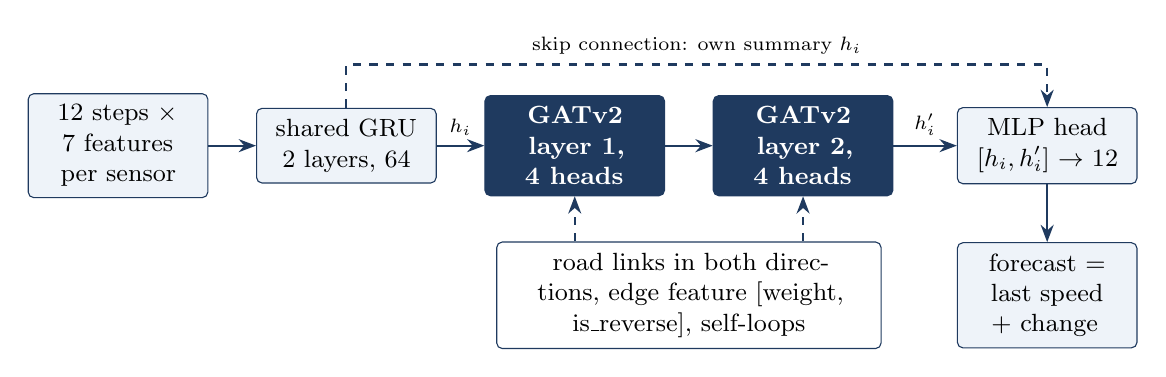
\begin{tikzpicture}[x=1cm,y=1cm]
\node[blk,text width=2.0cm] (in) at (1.1,0) {12 steps $\times$ 7 features per sensor};
\node[blk,text width=2.0cm] (gru) at (4.0,0) {shared GRU 2 layers, 64};
\node[dark,text width=2.0cm] (gat1) at (6.9,0) {GATv2 layer 1, 4 heads};
\node[dark,text width=2.0cm] (gat2) at (9.8,0) {GATv2 layer 2, 4 heads};
\node[blk,text width=2.0cm] (head) at (12.9,0) {MLP head $[h_i, h_i']\rightarrow 12$};
\node[blk,text width=4.6cm,fill=white] (edges) at (8.35,-1.9) {road links in both directions, edge feature [weight, is\_reverse], self-loops};
\node[blk,text width=2.0cm] (out) at (12.9,-1.9) {forecast = last speed + change};
\draw[arr] (in) -- (gru);
\draw[arr] (gru) -- node[above,font=\scriptsize]{$h_i$} (gat1);
\draw[arr] (gat1) -- (gat2);
\draw[arr] (gat2) -- node[above,font=\scriptsize]{$h_i'$} (head);
\draw[arr] (head) -- (out);
\draw[arr,dashed] (edges.north -| gat1) -- (gat1.south);
\draw[arr,dashed] (edges.north -| gat2) -- (gat2.south);
\draw[arr,dashed] (gru.north) -- ++(0,0.55) -| node[pos=0.25,above,font=\scriptsize]{skip connection: own summary $h_i$} (head.north);
\end{tikzpicture}
\caption{STGAT. A shared GRU summarises each sensor's history; two GATv2 layers mix each summary with its road
neighbours'; the head predicts the change from the last speed for all 12 horizons.}
\label{fig:stgat}
\end{figure}

\subsection{DCRNN: diffusion convolutional recurrent network}\label{sec:dcrnn}
Following~\citep{li2018dcrnn}, traffic is modelled as diffusion on the directed graph. With out- and in-degree matrices
$D_O, D_I$, the diffusion convolution of a signal $X$ is
\begin{equation}
X \star_{G} f_\theta = \sum_{k=0}^{K-1}\Bigl(\theta_{k,1}\bigl(D_O^{-1}W\bigr)^k + \theta_{k,2}\bigl(D_I^{-1}W^{\top}\bigr)^k\Bigr)X ,
\end{equation}
where the forward random walk mixes a sensor's upstream neighbours and the backward walk its downstream neighbours. The
diffusion convolution replaces every matrix product inside a GRU cell (DCGRU):
\begin{align}
r_t &= \sigma\bigl(\Theta_r\star_G[x_t,h_{t-1}] + b_r\bigr), \quad u_t = \sigma\bigl(\Theta_u\star_G[x_t,h_{t-1}] + b_u\bigr),\\
c_t &= \tanh\bigl(\Theta_c\star_G[x_t,\ r_t\odot h_{t-1}] + b_c\bigr), \quad h_t = u_t\odot h_{t-1} + (1-u_t)\odot c_t .
\end{align}
A two-layer DCGRU encoder (64 units, $K=2$) reads the 12 input steps; a two-layer DCGRU decoder emits the 12 forecasts
one at a time, trained with scheduled sampling~\citep{bengio2015scheduled}, which feeds the ground truth with a
probability that decays as training proceeds. Our port differs from the TensorFlow reference in two deliberate ways: the
Chebyshev-style recursion restarts for each support, and the $207\times207$ supports are dense matrices, cheaper than
sparse operations at this size.

\subsection{Hybrid: DCRNN with an XGBoost residual corrector}\label{sec:hybrid-method}
DCRNN is the strongest single model, but XGBoost, with calendar and segment features, remains slightly better at
60 minutes after a congestion onset, and the two err differently (Section~\ref{sec:where}). Following stacked
generalisation~\citep{wolpert1992stacking}, the hybrid keeps DCRNN as the backbone and learns its systematic error:
\begin{equation}
\hat y^{\,\mathrm{hyb}}_h = \hat y^{\,\mathrm{DCRNN}}_h + r_h\!\left(z,\ \hat y^{\,\mathrm{DCRNN}}_h,\ \hat y^{\,\mathrm{XGB}}_h\right),\qquad h=1,\dots,12,
\end{equation}
where $r_h$ is one shallow XGBoost model per horizon trained on the target $y_h-\hat y^{\,\mathrm{DCRNN}}_h$. Its inputs
are deliberately compact: the current speed, its change over 5 and 15 minutes, time of day, the weekend flag and the
sensor's free-flow speed, plus both forecasts, DCRNN's forecast minus the current speed, and the gap between the two
forecasts.

\textbf{Leakage rule.} The corrector must see DCRNN forecasts on data DCRNN was \emph{not} trained on, or it learns
in-sample residuals that are far too small. It is therefore fitted on the validation block, which DCRNN used only to
choose its best epoch: the first \HybFitWindows{} validation windows (75\%) fit $r_h$, the last \HybStopWindows{} decide
its early stopping, and the test block is scored exactly once. Two alternative designs serve as ablations: a per-horizon
convex blend of the two forecasts, and the same corrector on all 46 features with deeper trees.

\subsection{Training and regularisation}
All neural models minimise masked MAE in mph with Adam~\citep{kingma2015adam}, a step learning-rate schedule
($\times0.1$ at epochs 20 and 30), gradient clipping at norm 5, and early stopping on validation MAE with patience 8 that
never triggers before the last learning-rate drop. Each epoch draws a fresh random half of the training windows; windows
are shuffled only inside the training block. Table~\ref{tab:hparams} lists the settings.

\begin{table}[htbp]
\centering
\caption{Hyper-parameters. Graph models: main runs use seeds 0, 1, 2; ablations use seed 0 with the main run's budget.}
\label{tab:hparams}
\footnotesize
\begin{tabular}{@{}lll@{}}
\toprule
 & STGAT & DCRNN \\
\midrule
Parameters & \StgatParams & \DcrnnParams \\
Temporal unit & GRU, 2 layers, 64 units & DCGRU encoder--decoder, 2 layers, 64 units \\
Spatial unit & 2 GATv2 layers, 4 heads, edge features & diffusion, $K=2$, forward + backward walks \\
Regularisation & dropout 0.1, LayerNorm, residuals & scheduled sampling (decay 2000 batches) \\
Optimiser & Adam, lr $10^{-3}$, batch 32 & Adam, lr $10^{-2}$, batch 64 \\
Schedule & 40 epochs, lr $\times0.1$ at 20 and 30 & 30 epochs, lr $\times0.1$ at 20 and 30 \\
Early stopping & patience 8, after the last lr drop & patience 8, after the last lr drop \\
\midrule
\multicolumn{3}{@{}l}{\textbf{Hybrid corrector} (one XGBoost model per horizon): depth 3, $\geq$200 samples per leaf, L2 = 10,}\\
\multicolumn{3}{@{}l}{learning rate 0.03, subsample 0.8, column sample 0.8, MAE objective, up to 1\,500 rounds, early stopping 50.}\\
\bottomrule
\end{tabular}
\end{table}

\subsection{Verification of the implementation}
\NTests{} automated tests guard the pipeline and the models: chronological order and no shared target timestamps
between splits, train-only scaling, imputation that only looks back, masked targets contributing nothing to the loss,
sensor order matching the adjacency, the rebuilt adjacency equal to the supplied one, the attention layer equal to PyTorch
Geometric's \texttt{GATv2Conv}, information flowing only along the edges a model is given, the direction of each
diffusion support, and the hybrid's chronological fitting split. Regenerating the per-sensor baselines reproduces the
AML phase's numbers exactly.

%=====================================================================
\section{Experimental setup}\label{sec:setup}
\textbf{Runs.} STGAT and DCRNN are each trained with three seeds; we report the mean (and the standard deviation in the
appendix). The hybrid is built once on each DCRNN seed. Ablations (Section~\ref{sec:ablations}) change one component at
a time on seed 0 with the main run's budget. One extra DCRNN run uses the reference protocol (window-level split, scaler
including outage zeros) to compare with the published numbers.

\textbf{Metrics.} Masked MAE, RMSE and MAPE in mph (MAPE in percent) at every horizon; we quote 15, 30 and 60 minutes
(steps 3, 6 and 12). MAE is the headline: it is in the units a road user understands and is robust to rare large misses;
RMSE weighs those misses; MAPE expresses the error relative to the speed.

\textbf{Significance.} Errors within one day are strongly correlated, so the unit of resampling is the \emph{day}. For
each comparison and horizon we compute daily MAEs on the \TestDays{} test days and run (i) a paired bootstrap over days
with 10\,000 resamples and (ii) a Diebold--Mariano test on the daily loss differential with the Harvey--Leybourne--Newbold
small-sample correction. Each seed is tested separately and the \emph{worst} seed is reported.

\textbf{Hardware.} All models were trained on an Apple M3 Pro (Metal GPU); the full graph-model queue (main runs and
ablations) takes about 10 hours and is resumable.

%=====================================================================
\section{Results}\label{sec:results}

\subsection{Main comparison}
Table~\ref{tab:main} scores all ten models on the same test windows. Three findings stand out.
\begin{itemize}
\item \textbf{DCRNN is the best single model at every horizon}, at \DcrnnMAEFifteen{} / \DcrnnMAEThirty{} /
\DcrnnMAESixty\mph, \DcrnnGainFifteen\% / \DcrnnGainThirty\% / \DcrnnGainSixty\% below XGBoost.
\item \textbf{STGAT beats XGBoost clearly at short horizons} (\StgatGainFifteen\% at 15 minutes) but only by
\StgatGainSixty\% at 60 minutes, where it ties XGBoost with neighbour features.
\item \textbf{The hybrid is the best model overall}, with the lowest MAE and MAPE at every horizon:
\HybridMAEFifteen{} / \HybridMAEThirty{} / \HybridMAESixty\mph.
\end{itemize}
RMSE tells a more nuanced story. At 60 minutes DCRNN's RMSE (\DcrnnRMSESixty) is above XGBoost's (\XgbRMSESixty): it is
wrong less often, but its rarer misses, mostly when a jam starts, are larger. The hybrid reduces this to
\HybridRMSESixty, and XGBoost with neighbour features keeps the lowest RMSE at 30 and 60 minutes (\XgbNbRMSESixty{} at
60). A deployment that cares most about the worst errors should therefore keep a tree component, which is what the
hybrid does.

\begin{table}[htbp]
\centering
\caption{Test results (mph; MAPE in \%), by forecast horizon. Best value in each column in bold.
$^{\dagger}$Mean of 3 seeds. Above the line: per-sensor models from the AML phase; below: models of this phase.}
\label{tab:main}
\small
\setlength{\tabcolsep}{4.2pt}
\begin{tabular}{@{}lrrrrrrrrr@{}}
\toprule
 & \multicolumn{3}{c}{MAE} & \multicolumn{3}{c}{RMSE} & \multicolumn{3}{c}{MAPE (\%)} \\
\cmidrule(lr){2-4}\cmidrule(lr){5-7}\cmidrule(l){8-10}
Model & 15 & 30 & 60 & 15 & 30 & 60 & 15 & 30 & 60 \\
\midrule
\tabinput{generated/tab_main.tex}
\bottomrule
\end{tabular}
\end{table}

\begin{figure}[htbp]
\centering
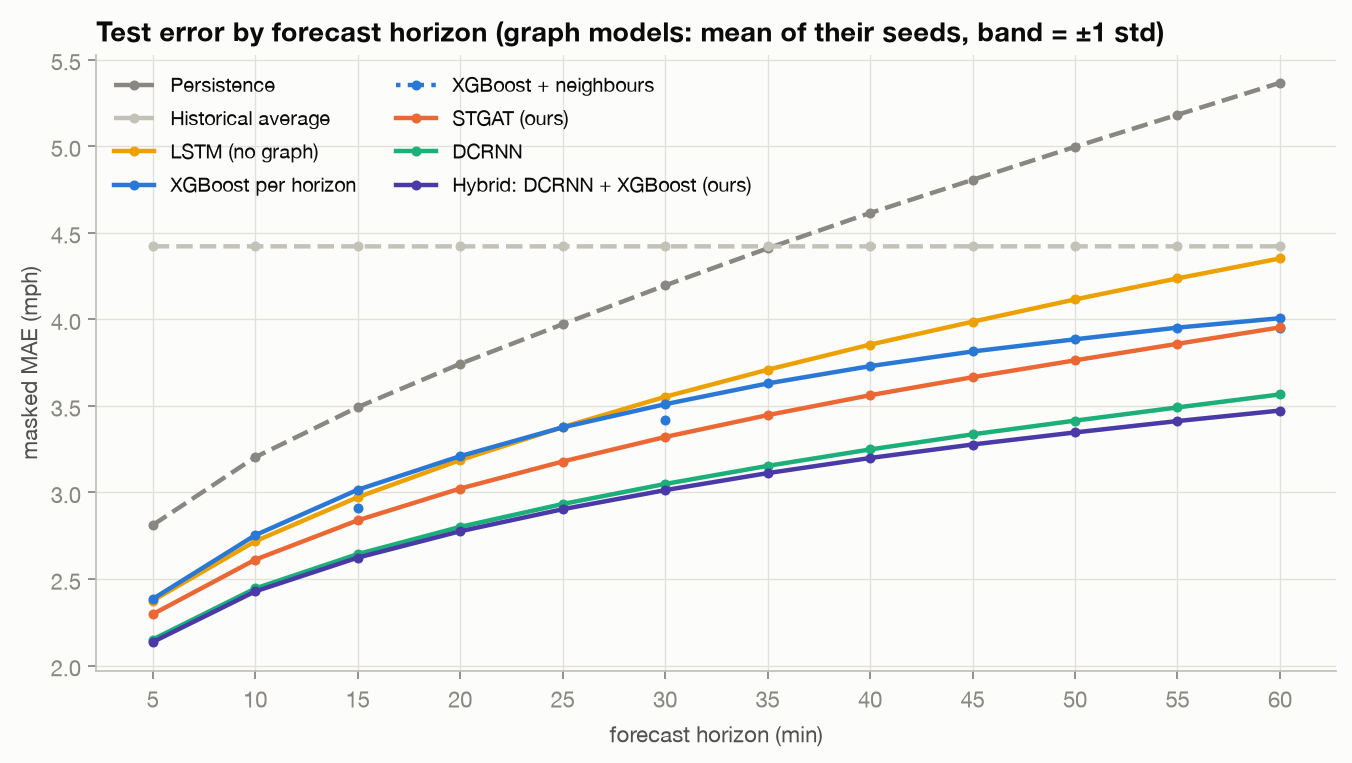
\includegraphics[width=0.88\linewidth]{fig15_final_error_by_horizon.png}
\caption{Test MAE at all 12 horizons. Graph models: mean of 3 seeds, band = $\pm$1 standard deviation. The graph models'
advantage holds from 5 to 60 minutes.}
\label{fig:horizon}
\end{figure}

\begin{table}[htbp]
\centering
\caption{Test MAE (mph) at all 12 horizons. Graph models and the hybrid: mean of 3 seeds. Best per row in bold.}
\label{tab:horizons}
\small
\begin{tabular}{@{}rrrrrrrr@{}}
\toprule
Step & Minutes & Persistence & LSTM (no graph) & XGBoost & STGAT & DCRNN & Hybrid \\
\midrule
\tabinput{generated/tab_horizons.tex}
\bottomrule
\end{tabular}
\end{table}

\subsection{Peak versus off-peak}
Weekday peak hours are where forecasts matter most and where every model is weakest: the 60-minute peak MAE is 1.76 to
1.95 times the off-peak MAE for every model (Table~\ref{tab:period}). The graph models help most exactly there: DCRNN's
peak-hour MAE is \PeakGainDcrnn\% below XGBoost's and the hybrid's \PeakGainHybrid\% below it (\HybridPeakSixty{}
against \XgbPeakSixty\mph). The hybrid is the best model in all three periods (Figure~\ref{fig:period}).

\begin{table}[htbp]
\centering
\caption{Test MAE (mph) at 60 minutes by period: weekday peak (07:00--09:59, 16:00--19:59), weekday off-peak and weekend.
Ratio = peak / off-peak. $^{\dagger}$Mean of 3 seeds.}
\label{tab:period}
\small
\begin{tabular}{@{}lrrrr@{}}
\toprule
Model & Peak & Off-peak & Weekend & Ratio \\
\midrule
\tabinput{generated/tab_period.tex}
\bottomrule
\end{tabular}
\end{table}

\begin{figure}[htbp]
\centering
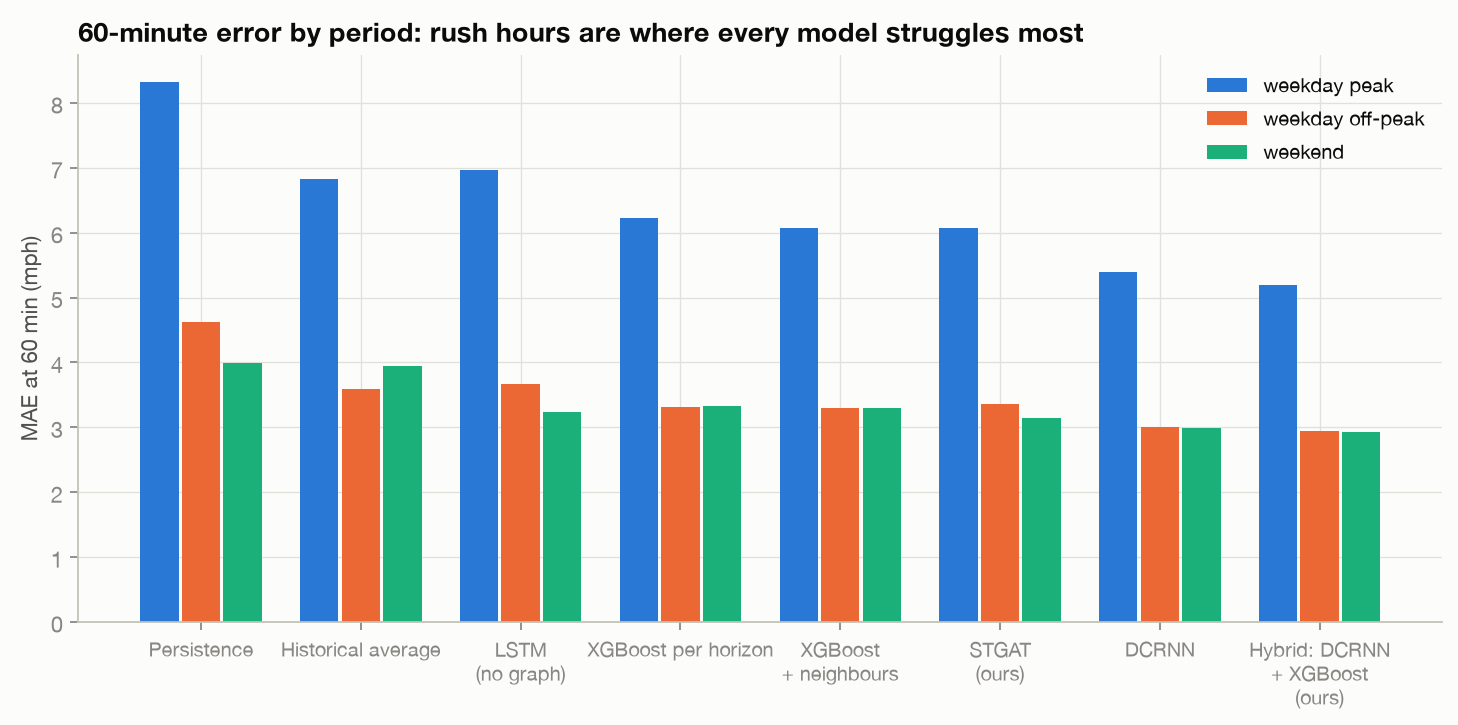
\includegraphics[width=0.86\linewidth]{fig16_final_peak_offpeak.png}
\caption{Peak, off-peak and weekend test MAE by horizon for the main models.}
\label{fig:period}
\end{figure}

\subsection{Statistical significance}
Table~\ref{tab:sig} reports the day-level tests. DCRNN and the hybrid beat XGBoost on all \TestDays{} test days at every
horizon. The hybrid beats DCRNN on at least \HybridMinDays{} of \TestDays{} days at every horizon, for every seed. STGAT's
15- and 30-minute gains are highly significant, but its 60-minute gain is weak (bootstrap $p$ = \StgatSixtyPBoot,
Diebold--Mariano $p$ = \StgatSixtyPDm, better on \StgatSixtyDays{} of \TestDays{} days).

\begin{table}[htbp]
\centering
\caption{Paired day-level tests over the \TestDays{} test days (worst of 3 seeds for $p$ and days; gain and interval:
mean of the per-seed values and their widest 95\% bootstrap interval). Gain = MAE reduction against the baseline.}
\label{tab:sig}
\footnotesize
\setlength{\tabcolsep}{3.5pt}
\begin{tabular}{@{}lrrrcrrr@{}}
\toprule
Comparison & Min & Gain (mph) & Gain (\%) & 95\% CI (mph) & Days & $p_{\text{boot}}$ & $p_{\text{DM}}$ \\
\midrule
\tabinput{generated/tab_sig.tex}
\bottomrule
\end{tabular}
\end{table}

\subsection{Reproducing the published DCRNN}
To check our port, we also trained DCRNN under the reference protocol: windows split 70/10/20 at window level and a
scaler that includes the outage zeros. This run stopped after 24 of its 30 epochs; we score its best checkpoint
(epoch 22, after the learning-rate drop). It reaches \RefFifteen{} / \RefThirty{} / \RefSixty\mph, within \RefWorstPct\%
of the published values~\citep{li2018dcrnn} (Table~\ref{tab:reference}). Under the strict protocol used everywhere else
the numbers are of the same size: the stricter split costs about half a percent but removes the overlap between training
and validation targets.

\begin{table}[htbp]
\centering
\caption{DCRNN test MAE (mph): published, our port under the reference protocol, and our port under the strict protocol (mean of 3 seeds).}
\label{tab:reference}
\small
\begin{tabular}{@{}rrrrr@{}}
\toprule
Minutes & Published~\citep{li2018dcrnn} & Ours, reference protocol & Difference (\%) & Ours, strict protocol \\
\midrule
\tabinput{generated/tab_reference.tex}
\bottomrule
\end{tabular}
\end{table}

\subsection{Training behaviour and seed stability}
Figure~\ref{fig:curves} shows the learning curves. DCRNN's validation error at the initial learning rate of 0.01 is noisy,
with spikes in the first epochs, and settles sharply at the first learning-rate drop (epoch 20); this is why early
stopping never triggers before the last drop. STGAT improves smoothly. Neither model overfits: validation error flattens without rising. Results are very stable across seeds
(Table~\ref{tab:seeds}): the seed standard deviation is at most 0.002\mph{} for STGAT and 0.010\mph{} for DCRNN, far below
every difference discussed in this report.

\begin{figure}[htbp]
\centering
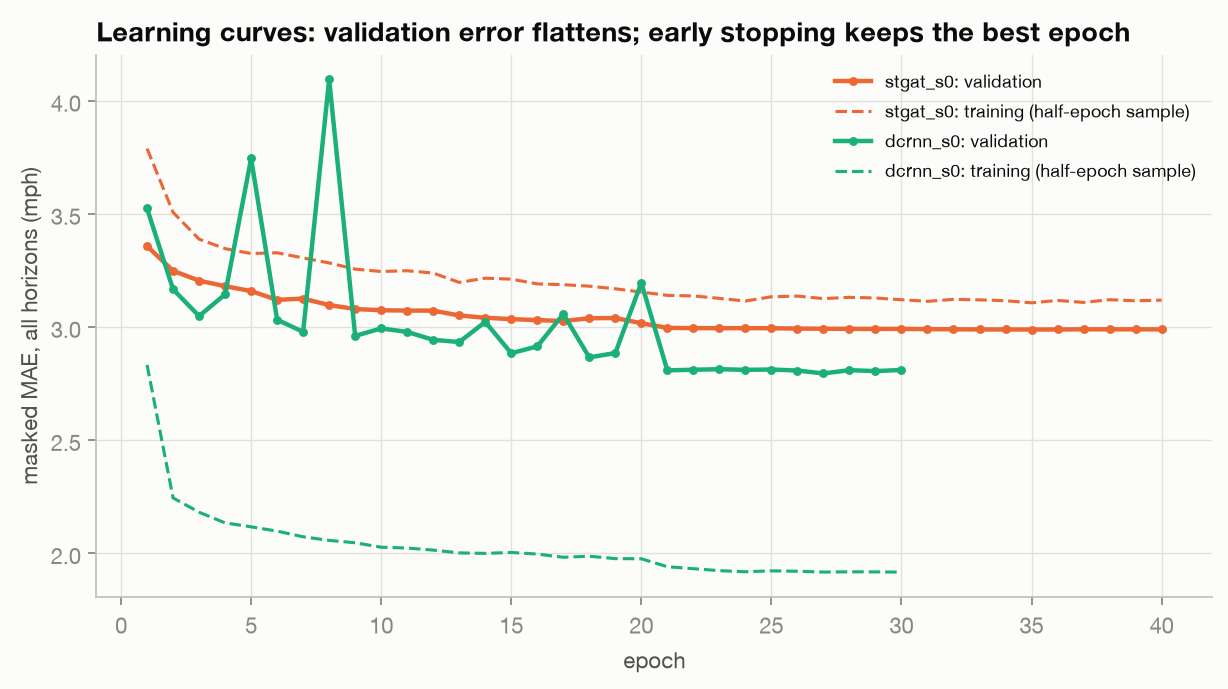
\includegraphics[width=0.9\linewidth]{fig12_learning_curves.png}
\caption{Training and validation MAE per epoch for STGAT and DCRNN (seed 0).}
\label{fig:curves}
\end{figure}

%=====================================================================
\section{Analysis: where the gain comes from}\label{sec:analysis}

\subsection{Ablations}\label{sec:ablations}
Table~\ref{tab:ablation} changes one component at a time (Figure~\ref{fig:ablation}).
\begin{itemize}
\item \textbf{No graph.} With self-loops only, STGAT falls back to the level of the no-graph LSTM (\AblNoGraphSixty\mph{}
at 60 minutes, +\AblNoGraphDelta): the gain comes from the neighbours, not from the architecture.
\item \textbf{Random graph.} A graph with as many random links and shuffled real weights is clearly worse
(+\AblRandomDelta\mph): the \emph{road} structure matters, not just extra inputs.
\item \textbf{Direction.} Downstream-only messages (+\AblBwdDelta) beat upstream-only messages (+\AblFwdDelta), and both
directions are best, exactly as the measured backward propagation predicts. Dropping the direction feature also costs
(+\AblUndirDelta). DCRNN shows the same: without its backward random walk the 60-minute MAE rises by \AblDcrnnFwdDelta\mph.
\item \textbf{Hops.} One attention layer instead of two costs +\AblOneLayerDelta\mph; one diffusion hop instead of two
barely changes DCRNN (+\AblDcrnnKoneDelta), because its recurrence already propagates information at every step.
\item \textbf{Regularisation.} Removing dropout changes STGAT by \AblNoDropDelta\mph: with \StgatParams{} parameters and
22\,933 training windows it does not overfit, so early stopping and layer normalisation suffice.
\end{itemize}

\begin{table}[htbp]
\centering
\caption{Ablations: test MAE (mph), seed 0. $\Delta_{60}$ = change at 60 minutes against the main run of the same model.}
\label{tab:ablation}
\small
\begin{tabular}{@{}lrrrrr@{}}
\toprule
Variant & Parameters & 15 & 30 & 60 & $\Delta_{60}$ \\
\midrule
\tabinput{generated/tab_ablation.tex}
\bottomrule
\end{tabular}
\end{table}

\begin{figure}[htbp]
\centering
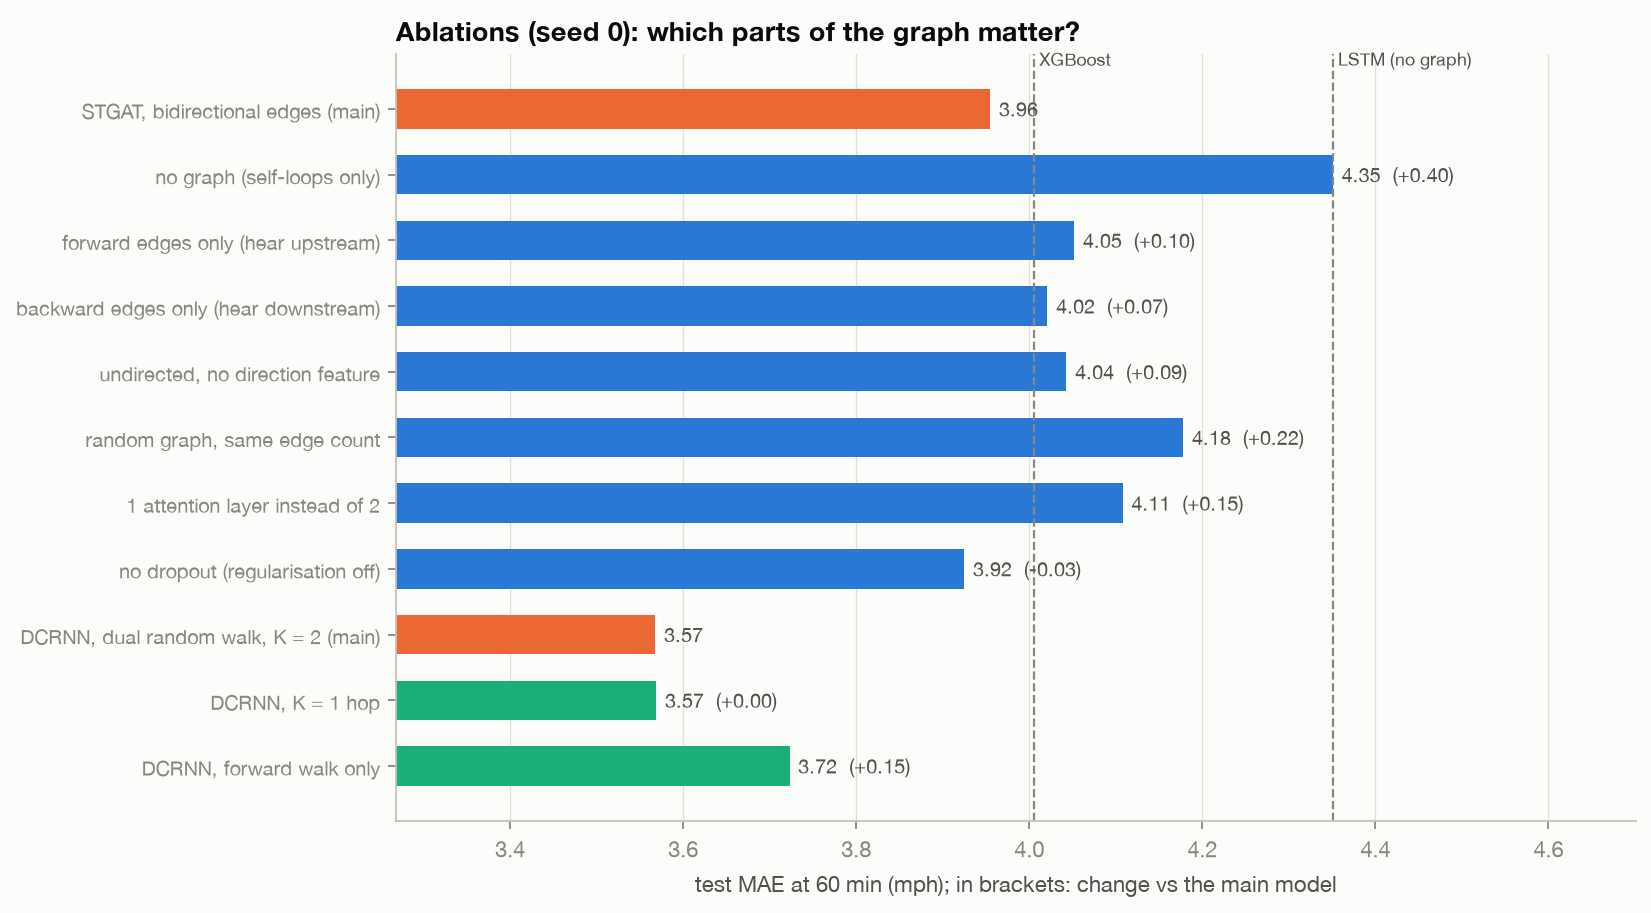
\includegraphics[width=0.9\linewidth]{fig13_ablations.png}
\caption{Ablations at 60 minutes: change in test MAE against the main run of each model.}
\label{fig:ablation}
\end{figure}

\subsection{The hybrid}\label{sec:hybrid}
Table~\ref{tab:hybrid} compares hybrid designs on the same three DCRNN seeds. A per-horizon blend helps a little (its
optimal weight on DCRNN is \BlendWFifteen{} at 15 and \BlendWSixty{} at 60 minutes). A residual corrector on all 46
features with deep trees \emph{overfits} the short fitting block and is worse than DCRNN alone at 30 and 60 minutes. The
compact, regularised corrector improves DCRNN at every horizon, most at 60 minutes (\HybridOverDcrnnSixty\%), where
calendar knowledge matters most. Regularisation matters where data are scarce: here, not in the graph models.

What the corrector uses is telling (Table~\ref{tab:corrector}): the single most important input is the \emph{disagreement}
between the two forecasts (\CorrTopShare\% of the gain), followed by time of day and the weekend flag, whose share grows
with the horizon. The corrector learns when to trust the tree's calendar view over the graph's spatial view.

\begin{table}[htbp]
\centering
\caption{Hybrid designs: test MAE (mph), mean $\pm$ standard deviation over the 3 DCRNN seeds. Best in bold.}
\label{tab:hybrid}
\small
\begin{tabular}{@{}lrrr@{}}
\toprule
Design & 15 min & 30 min & 60 min \\
\midrule
\tabinput{generated/tab_hybrid.tex}
\bottomrule
\end{tabular}
\end{table}

\begin{table}[htbp]
\centering
\caption{Inputs of the hybrid corrector: share of total split gain (\%), mean over the 3 seeds, overall and at 15, 30 and 60 minutes.}
\label{tab:corrector}
\small
\begin{tabular}{@{}lrrrr@{}}
\toprule
Input & All horizons & 15 min & 30 min & 60 min \\
\midrule
\tabinput{generated/tab_corrector.tex}
\bottomrule
\end{tabular}
\end{table}

\subsection{Where in the network and when the graph helps}\label{sec:where}
\textbf{Connectivity.} The gain of DCRNN over XGBoost at 60 minutes grows with a sensor's number of road links, from
\DegGainLow\% for sensors with 0--4 links to \DegGainHigh\% for sensors with 13 or more (Table~\ref{tab:degree}). STGAT is
slightly worse than XGBoost on the 15 sparsely connected sensors, where it has few neighbours to listen to.

\textbf{Congestion onsets.} In the 30 minutes after a congestion onset (\OnsetTargets{} test targets), DCRNN's 15-minute
error is \OnsetDcrnnFifteen\mph{} against \OnsetXgbFifteen\mph{} for XGBoost (Table~\ref{tab:onset}): it sees the slowdown
at a neighbour first. At 60 minutes ahead the jam usually has not started anywhere yet, and XGBoost's calendar knowledge
is slightly better (\OnsetXgbSixty{} against \OnsetDcrnnSixty): the complementarity the hybrid exploits, bringing the
60-minute onset error down to \OnsetHybridSixty.

\begin{table}[htbp]
\centering
\caption{Test MAE (mph) at 60 minutes by sensor connectivity (number of road links). Gain = DCRNN versus XGBoost.}
\label{tab:degree}
\small
\begin{tabular}{@{}lrrrrrr@{}}
\toprule
Links & Sensors & XGBoost & STGAT & DCRNN & Hybrid & DCRNN gain (\%) \\
\midrule
\tabinput{generated/tab_degree.tex}
\bottomrule
\end{tabular}
\end{table}

\begin{table}[htbp]
\centering
\caption{Test MAE (mph) in the 30 minutes after a congestion onset and at all other times. Best onset value per horizon in bold.}
\label{tab:onset}
\small
\begin{tabular}{@{}lrrrrrr@{}}
\toprule
 & \multicolumn{3}{c}{After an onset} & \multicolumn{3}{c}{Other times} \\
\cmidrule(lr){2-4}\cmidrule(l){5-7}
Model & 15 & 30 & 60 & 15 & 30 & 60 \\
\midrule
\tabinput{generated/tab_onset.tex}
\bottomrule
\end{tabular}
\end{table}

\begin{figure}[htbp]
\centering
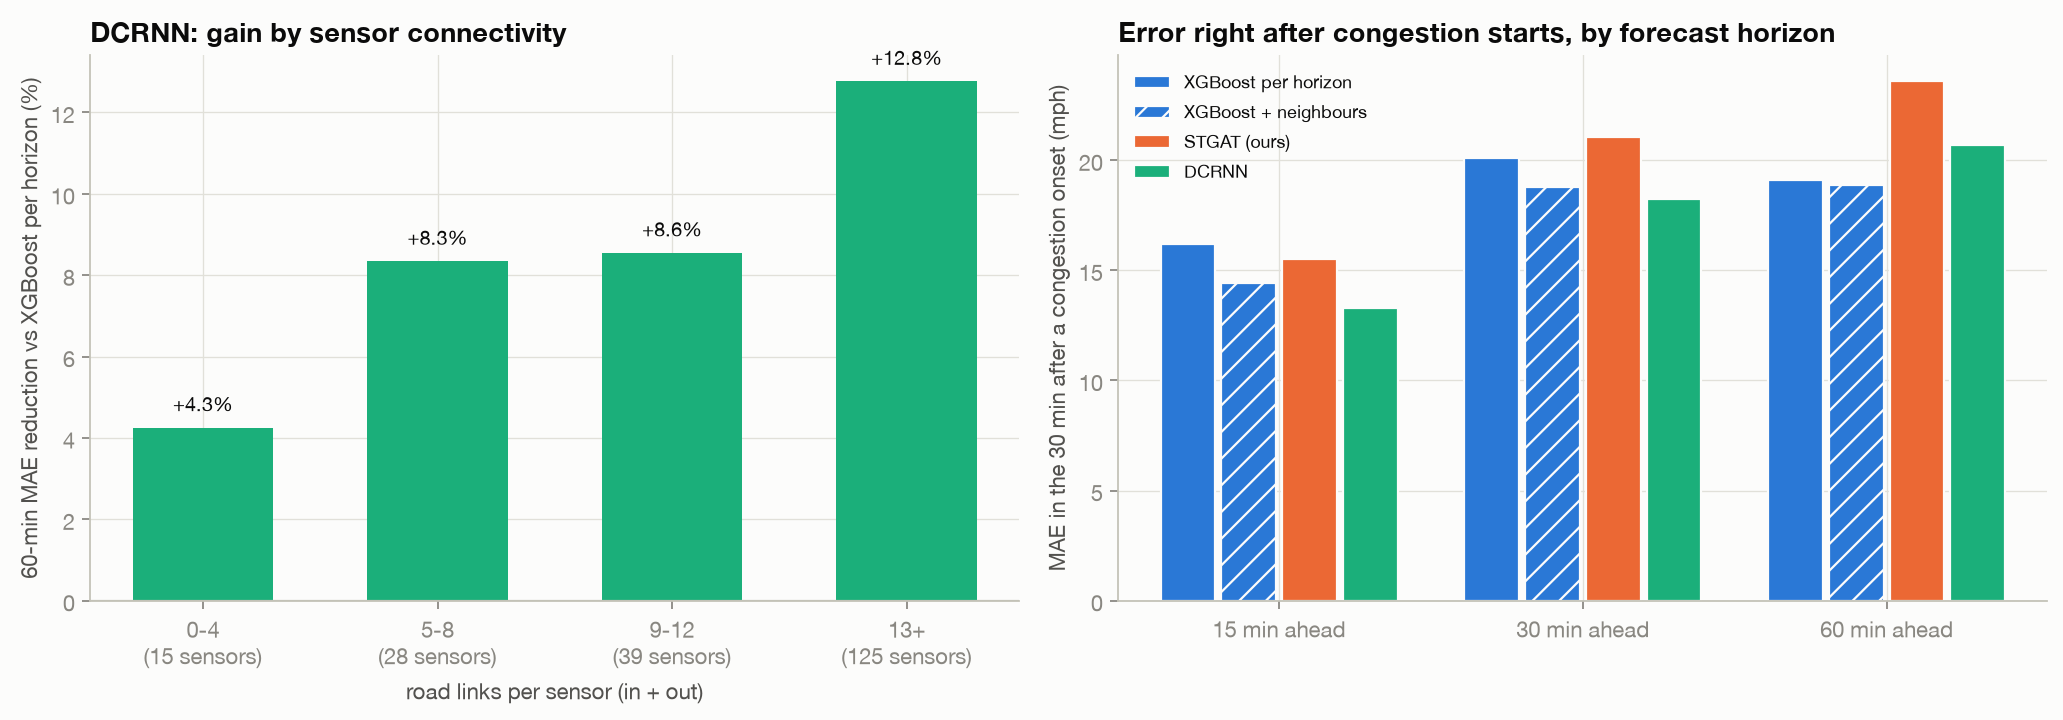
\includegraphics[width=0.92\linewidth]{fig17_where_the_graph_helps.png}
\caption{Where the graph helps: gain by sensor connectivity (left) and error after congestion onsets (right).}
\label{fig:where}
\end{figure}

\subsection{What the attention learned}
We inspected the last attention layer of STGAT on the test block for the \AttSensors{} sensors that have both upstream
and downstream neighbours, comparing the \AttWindows{} windows in which the sensor slows down within 30 minutes with all
other windows (Table~\ref{tab:attention}, Figure~\ref{fig:attention}). In normal windows a sensor gives \AttDownNormal\%
of its attention to downstream neighbours; when a slowdown is approaching this rises to \AttDownAhead\%, and
\AttShifted{} of the \AttSensors{} sensors shift downstream. Nothing in the model says ``look downstream'': it learned the
direction that the data analysis found.

\begin{table}[htbp]
\centering
\caption{Mean share of STGAT's attention (\%), \AttSensors{} sensors, test block.}
\label{tab:attention}
\small
\begin{tabular}{@{}lrrr@{}}
\toprule
Situation & Self & Upstream neighbours & Downstream neighbours \\
\midrule
\tabinput{generated/tab_attention.tex}
\bottomrule
\end{tabular}
\end{table}

\begin{figure}[htbp]
\centering
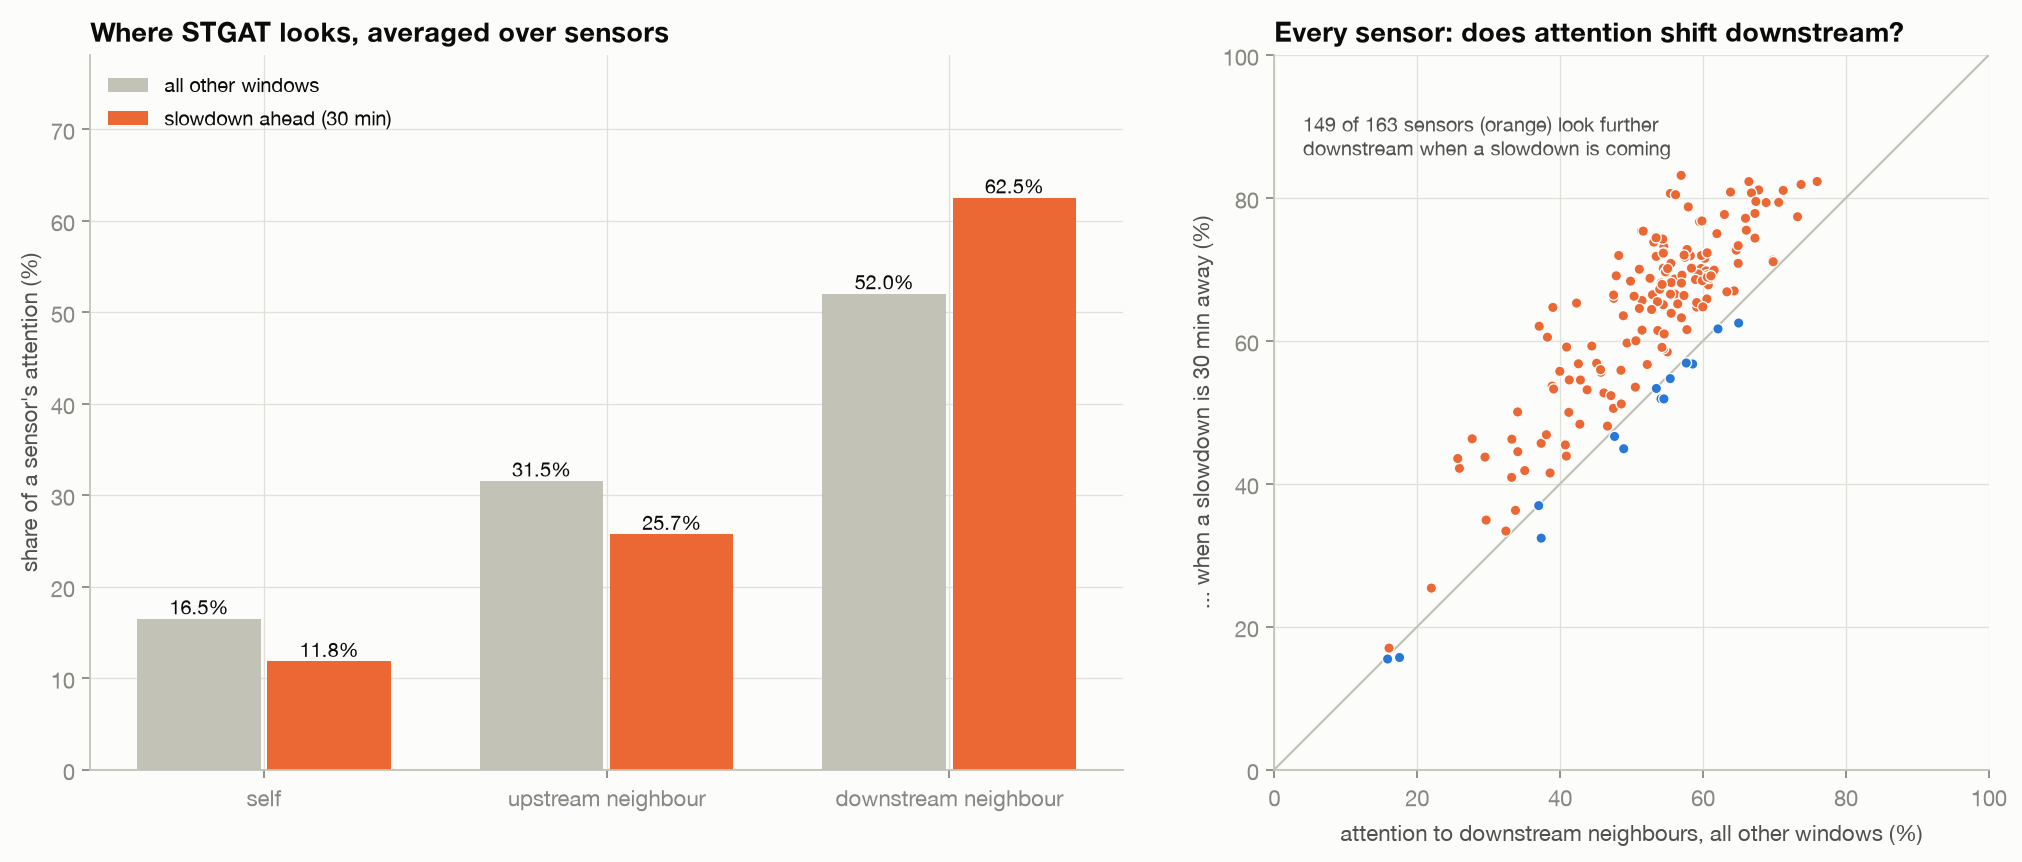
\includegraphics[width=0.9\linewidth]{fig14_attention.png}
\caption{STGAT attention by situation. When a slowdown is 30 minutes away, attention moves to downstream neighbours.}
\label{fig:attention}
\end{figure}

%=====================================================================
\section{Congestion maps}\label{sec:maps}
The brief's expected deliverable is a forecast comparison with congestion maps. Congestion level is speed divided by the
sensor's free-flow speed (the 85th percentile of its training speeds).

\textbf{Side-by-side map.} At the busiest weekday PM-peak test moment (\MapTime, chosen by that rule rather than by which
model looks better), \MapCongested{} sensors were congested. The 30-minute forecasts of XGBoost caught \MapXgbCaught{} of
them, DCRNN \MapGraphCaught; DCRNN placed \MapGraphLevel\% of all sensors in the right congestion level against
\MapXgbLevel\% for XGBoost (Figure~\ref{fig:map}).

\textbf{Error map.} Over the whole test block DCRNN has the lower 60-minute error at \MapSensorsBetter{} of 207 sensors,
with a median gain of \MapMedianGain\mph{} per sensor (Figure~\ref{fig:errmap}); the largest gains lie along the main
freeway corridors, and the few sensors where XGBoost is better sit at the edges of the network, including the isolated sensor.

\textbf{Time--space diagram.} Figure~\ref{fig:ts} follows \TsSensors{} consecutive sensors over \TsKm~km of one freeway
on \TsDay: the evening jam starts at the downstream end and spreads backwards (upstream) over time. Forecasting
30 minutes ahead, DCRNN reproduces the start of the jam and its upstream spread more closely than XGBoost, whose jam
starts later and is weaker, although DCRNN over-extends the jam on part of the corridor. An animated congestion map is included as
\texttt{docs/figures/fig21\_congestion\_animation.html}.

\begin{figure}[htbp]
\centering
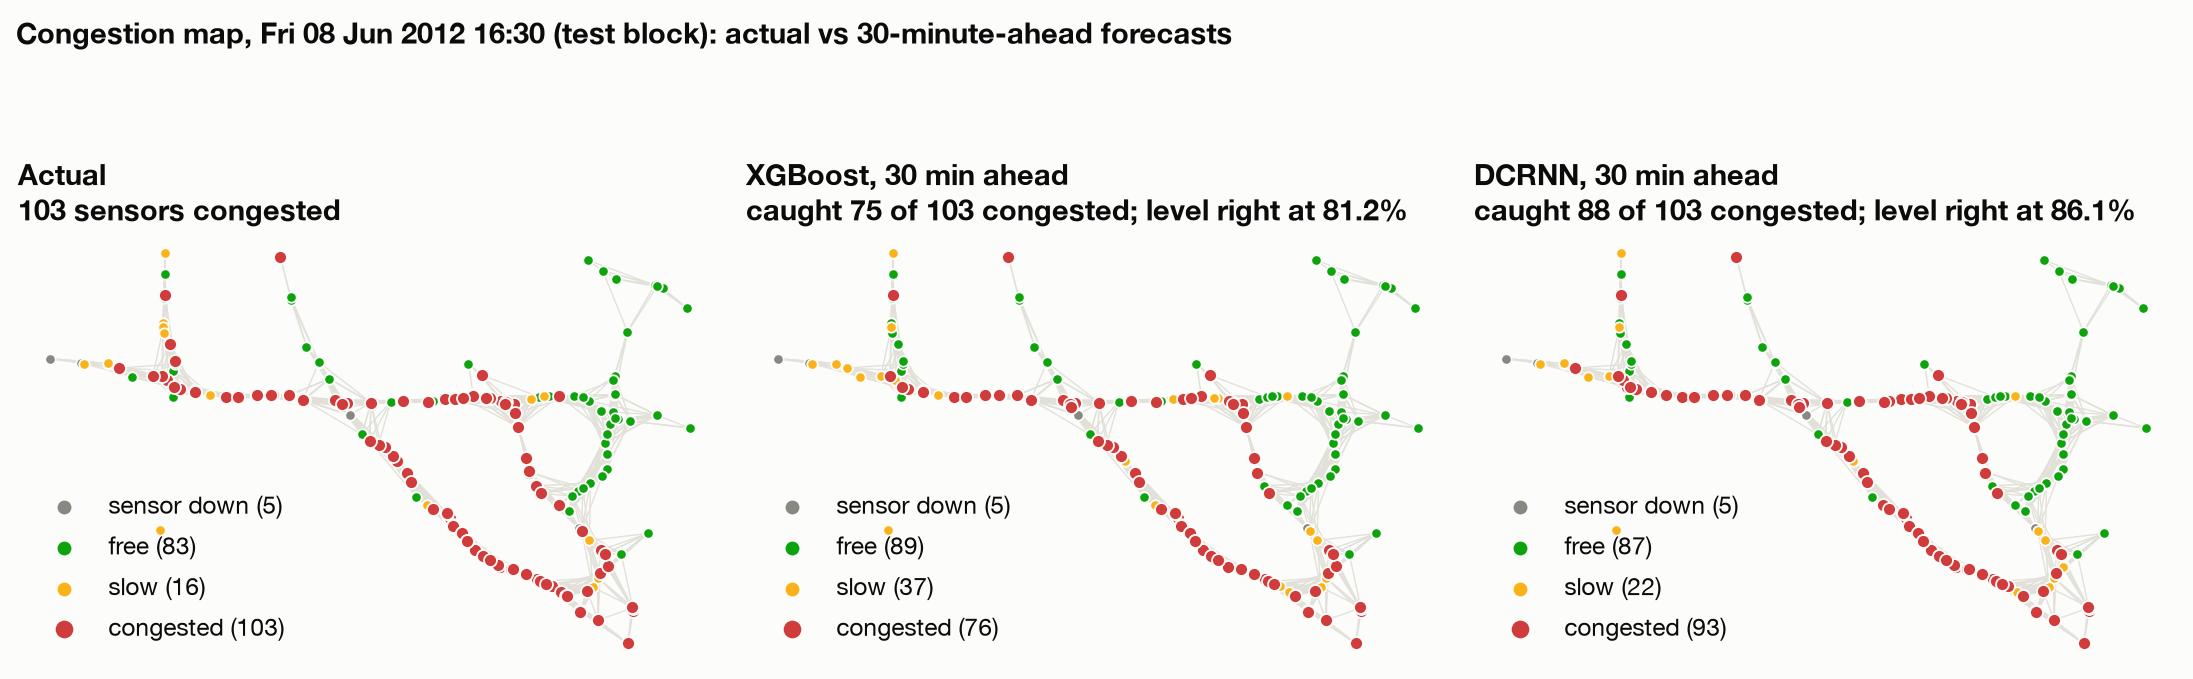
\includegraphics[width=\linewidth]{fig18_congestion_map_side_by_side.png}
\caption{Congestion levels at a PM-peak test moment: actual, and 30-minute forecasts by XGBoost and DCRNN.}
\label{fig:map}
\end{figure}

\begin{figure}[htbp]
\centering
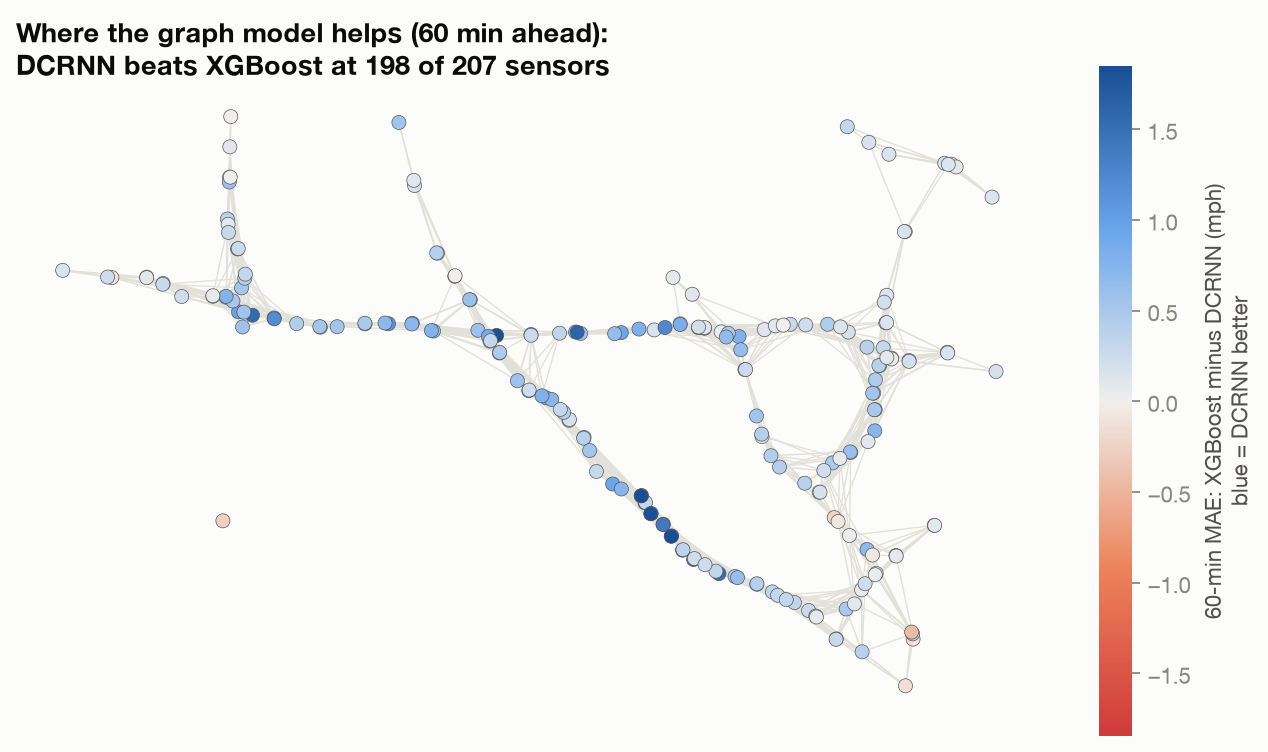
\includegraphics[width=0.78\linewidth]{fig19_error_map.png}
\caption{Error map: 60-minute MAE of XGBoost minus DCRNN per sensor over the test block (positive = DCRNN better).}
\label{fig:errmap}
\end{figure}

\begin{figure}[htbp]
\centering
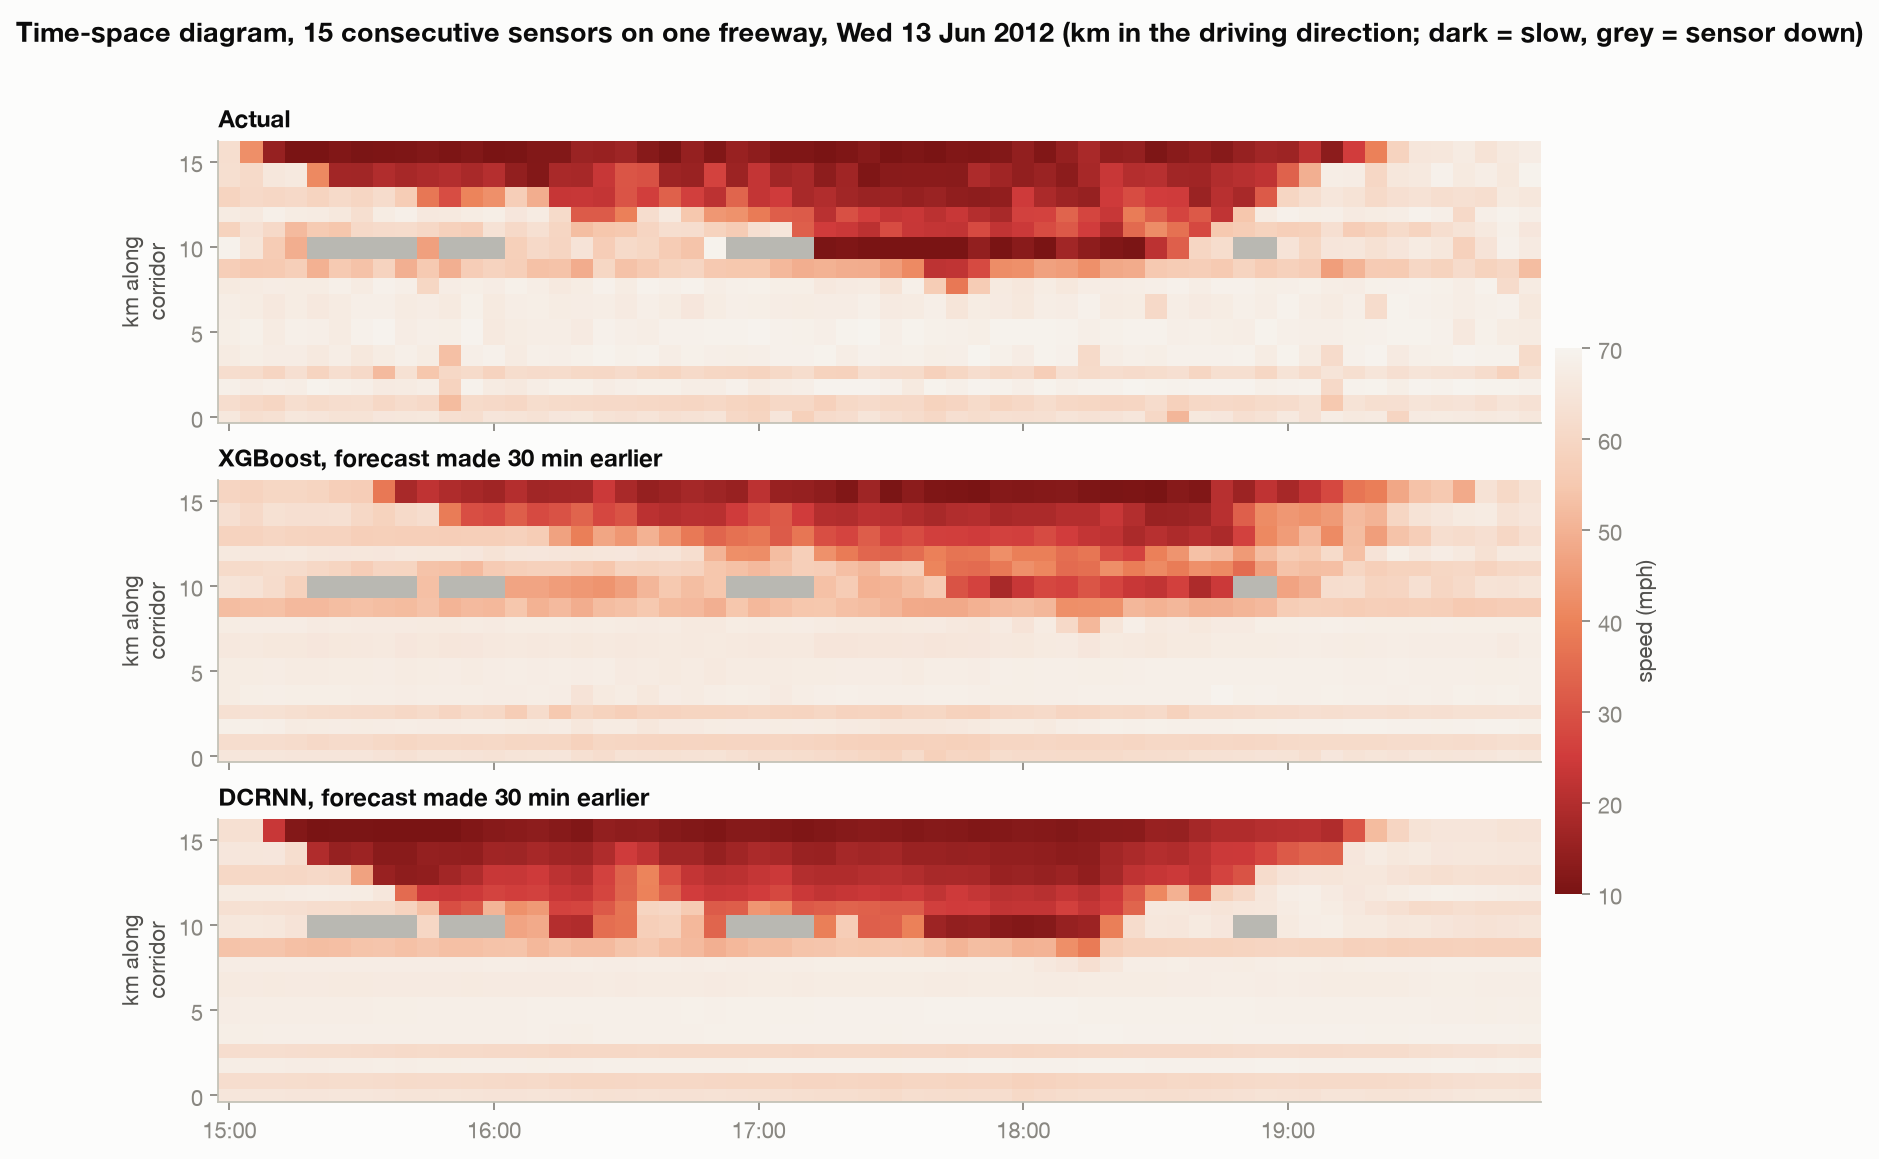
\includegraphics[width=\linewidth]{fig20_time_space_diagram.png}
\caption{Time--space diagram along one freeway on \TsDay: actual speeds and 30-minute forecasts.}
\label{fig:ts}
\end{figure}

%=====================================================================
\section{Outcomes}\label{sec:outcomes}

\subsection{Hypotheses revisited}
\begin{table}[H]
\centering
\caption{Hypotheses of the DL phase and their outcome.}
\label{tab:hyp}
\small
\begin{tabularx}{\linewidth}{@{}lXl@{}}
\toprule
 & Hypothesis and evidence & Outcome \\
\midrule
H5 & A graph model beats the best per-sensor model at every horizon. DCRNN: $-$\DcrnnGainFifteen\% / $-$\DcrnnGainThirty\% / $-$\DcrnnGainSixty\% MAE, all \TestDays{} days, $p<0.0001$ (Table~\ref{tab:sig}). STGAT: significant at 15 and 30 minutes, weak at 60. & \textcolor{good}{\textbf{Supported}} \\
H6 & The gain comes from the real road graph. No graph: +\AblNoGraphDelta\mph; random graph: +\AblRandomDelta\mph{} at 60 minutes (Table~\ref{tab:ablation}). & \textcolor{good}{\textbf{Supported}} \\
H7 & Downstream information is worth more than upstream. Backward-only beats forward-only edges; DCRNN without the backward walk loses \AblDcrnnFwdDelta\mph; attention shifts downstream before slowdowns. & \textcolor{good}{\textbf{Supported}} \\
H8 & The gain is larger for well-connected sensors and after congestion onsets. Gain grows from \DegGainLow\% to \DegGainHigh\% with connectivity; after onsets DCRNN is far better at 15 and 30 minutes but not at 60. & \textcolor{warn}{\textbf{Partly supported}} \\
H9 & Graph and tree models are complementary. The leak-free hybrid improves on DCRNN at every horizon (\HybridOverDcrnnSixty\% at 60 minutes), on at least \HybridMinDays{} of \TestDays{} days. & \textcolor{good}{\textbf{Supported}} \\
\bottomrule
\end{tabularx}
\end{table}

\subsection{Requirements of the brief}
\begin{table}[H]
\centering
\caption{Coverage of the project brief (AML and DL phases together).}
\label{tab:brief}
\small
\begin{tabularx}{\linewidth}{@{}p{4.6cm}Xl@{}}
\toprule
Requirement & Where it is delivered & Status \\
\midrule
Predict congestion in a road network & 207 sensors, 5 to 60 minutes ahead, all models & \textcolor{good}{Done} \\
Test whether graph learning beats independent segment forecasts & Tables~\ref{tab:main}, \ref{tab:sig}; ablations & \textcolor{good}{Done} \\
AML baseline: lagged speed, time of day, segment features; XGBoost per segment or multi-output RF & AML phase: 46 features, XGBoost per horizon, multi-output RF and four more baselines & \textcolor{good}{Done} \\
Flow and occupancy features & METR-LA records speed only; requires PeMS & \textcolor{warn}{Not available} \\
Identify the gap & AML phase: four gap experiments (Section~\ref{sec:aml}) & \textcolor{good}{Done} \\
GAT or diffusion graph model over a fixed adjacency & STGAT (GATv2) and DCRNN, both on the fixed METR-LA graph & \textcolor{good}{Done (both)} \\
Chronological splits; MAE, RMSE, MAPE by horizon & Section~\ref{sec:data}; Tables~\ref{tab:main}, \ref{tab:horizons} & \textcolor{good}{Done} \\
Equal history windows & 12 steps (60 minutes) for every model & \textcolor{good}{Done} \\
Peak versus off-peak & Table~\ref{tab:period}, Figure~\ref{fig:period} & \textcolor{good}{Done} \\
Adjacency from the supplied graph; train-only scaling; cyclic time; no random split; masked outages & Section~\ref{sec:data}, enforced by \NTests{} tests & \textcolor{good}{Done} \\
Forecast comparison with congestion maps & Section~\ref{sec:maps}, Figures~\ref{fig:map}--\ref{fig:ts} & \textcolor{good}{Done} \\
Optional simulated signal-policy experiment (SUMO) & Not run; freeways have no signals (Section~\ref{sec:limits}) & \textcolor{warn}{Not done} \\
\bottomrule
\end{tabularx}
\end{table}

%=====================================================================
\section{Discussion and limitations}\label{sec:discussion}

\subsection{Why DCRNN beats STGAT}
Where the graph enters the model matters. DCRNN mixes neighbours at every recurrent step of both encoding and decoding,
so information can travel several links during a forecast; STGAT summarises each sensor first and mixes once. DCRNN's
advantage therefore persists at long horizons, while STGAT's fades. STGAT is, however, more than five times smaller and
its attention is directly interpretable, which DCRNN's diffusion weights are not.

\subsection{Average error versus worst errors}
A lower MAE does not mean fewer large misses: at 60 minutes DCRNN's RMSE is above XGBoost's. The graph model is better
almost everywhere but occasionally misjudges the timing of a jam by a large margin. A system that must avoid the worst
errors should combine the two views, which is what the hybrid does.

\subsection{Limitations}\label{sec:limits}
\begin{itemize}
\item \textbf{Speed only.} METR-LA records speed; flow and occupancy features, named in the brief, need PeMS data.
\item \textbf{One city, one period.} The data are 2012 freeway readings from Los Angeles; transfer to other networks is untested.
\item \textbf{Seeds.} Main graph models and the hybrid use 3 seeds; ablations use one seed, and the per-sensor baselines were trained once.
\item \textbf{Validation reuse.} The hybrid is fitted on the validation block, which the per-sensor baselines did not use for fitting.
\item \textbf{Fixed graph.} The adjacency is fixed; a learned adjacency (as in Graph WaveNet) is a natural extension.
\item \textbf{No signal control.} The optional signal-control experiment was not run: METR-LA freeways have no traffic
signals, so it would require a simulation of a synthetic network in SUMO or CityFlow. Nothing in this project controls,
or claims to control, real traffic.
\end{itemize}

%=====================================================================
\section{Conclusion and future work}\label{sec:conclusion}
Under a strict, shared protocol, graph neural networks close a real part of the spatial gap left by per-sensor models.
DCRNN improves on a tuned XGBoost by 11--13\% at every horizon and on every test day; the gain grows with connectivity,
is largest right after congestion starts and at peak hours, and depends on the real road graph and on listening
downstream, which the trained attention confirms. A compact, regularised tree corrector, fitted without touching the test
data, adds a further, significant gain on top of the graph model, combining the graph's spatial view with the trees'
calendar knowledge into the best model of the project.

\textbf{Future work.} (i) Extend to PeMS-BAY and PeMS districts with flow and occupancy; (ii) learn the adjacency or add
temporal attention (Graph WaveNet, GMAN); (iii) per-step attention in STGAT at a higher compute budget; (iv) probabilistic
forecasts to address the large-miss problem directly; (v) a simulation-only signal-control study on a synthetic arterial
network, using the forecasts as inputs to a reinforcement-learning controller in CityFlow or SUMO.

%=====================================================================
\section*{Team contributions}
\addcontentsline{toc}{section}{Team contributions}
Each member owns parts of both the machine-learning phase and the deep-learning phase.
\begin{table}[H]
\centering
\small
\begin{tabularx}{\linewidth}{@{}lXX@{}}
\toprule
Member & AML phase & DL phase \\
\midrule
Harsh Raj (2401010180) & project setup, data loading, exploratory analysis, congestion-propagation finding & STGAT graph attention model, graph layers, attention inspection \\
Manas Saxena (2401010260) & leak-free preprocessing, the six baselines, XGBoost and Random Forest tuning, AML report and slides & fair comparison and day-level significance tests, hybrid DCRNN + XGBoost model, published-number reproduction, this report \\
Adil Mirza (2401020005) & feature engineering & DCRNN model, ablation studies \\
Augustya Purohit (2401010114) & gap analysis: horizon, onset, residual and neighbour experiments & IEEE research paper \\
Sumit Yadav (2401010464) & Streamlit dashboard and accuracy metrics & congestion maps, time--space diagram, DL slides \\
\bottomrule
\end{tabularx}
\end{table}

\FloatBarrier
\bibliographystyle{plainnat}
\bibliography{references}

%=====================================================================
\clearpage
\appendix
\section{Per-seed results of the graph models}\label{app:seeds}
\begin{table}[htbp]
\centering
\caption{Every main run: parameters, epochs run, best epoch, best validation MAE and test MAE (mph).}
\label{tab:seeds}
\small
\begin{tabular}{@{}lrrrrrrrr@{}}
\toprule
Model & Seed & Parameters & Epochs & Best epoch & Val MAE & Test 15 & Test 30 & Test 60 \\
\midrule
\tabinput{generated/tab_seeds.tex}
\bottomrule
\end{tabular}
\end{table}

\section{Reproducing this report}\label{app:repro}
\begin{tabularx}{\linewidth}{@{}>{\ttfamily\small}p{5.6cm}X@{}}
\toprule
\normalfont\textbf{Command} & \textbf{What it does} \\
\midrule
make setup data & environment, METR-LA download and the sensor graph \\
make preprocess features & leak-free windows and the per-sensor feature tables \\
make baselines gap & per-sensor baselines and gap experiments (AML phase) \\
make graph & STGAT and DCRNN, 3 seeds, ablations and the reference run (about 10 h, resumable) \\
make hybrid & DCRNN + XGBoost residual corrector and its ablations \\
make phase5 compare maps & ablation table, attention, final comparison, significance tests, maps \\
make dl-report & regenerate this report's tables from \texttt{results/} and compile it \\
\bottomrule
\end{tabularx}

\section{Traceability}
Every table and quoted number in this report is generated by \texttt{scripts/make\_dl\_report\_tables.py} from the
following files in \texttt{results/}:
\begin{itemize}
\item \texttt{final.csv}, \texttt{final\_by\_horizon.csv}: main comparison, all horizons, peak and off-peak;
\item \texttt{significance.csv}: day-level bootstrap and Diebold--Mariano tests;
\item \texttt{ablations.csv}, \texttt{graph\_models.csv}, \texttt{graph/*.json}: ablations, per-seed runs, training histories;
\item \texttt{hybrid\_ablation.csv}, \texttt{hybrid.json}, \texttt{hybrid/corrector\_importance\_s*.csv}: the hybrid;
\item \texttt{gain\_by\_degree.csv}, \texttt{gain\_at\_onset.csv}, \texttt{attention\_shares.csv}: where the graph helps, attention;
\item \texttt{phase1\_findings.json} to \texttt{phase7\_maps.json}: data facts, reference check, maps.
\end{itemize}
Figures are produced by \texttt{src/eval/phase5.py}, \texttt{src/eval/compare.py} and \texttt{src/viz/maps.py}; the split
table is shared with the AML report.

\end{document}
